% The title slide

changequote([[[, ]]])

\begin{slide}
\centerslidestrue
\begin{center}
\title{\LARGE Unix/Linux Programming in C}
\author{(NSWI015)}
\date{Version: \rm\today}
\maketitle

% \v{c} - hacek nad c
% \'{y} - carka nad y
% \'{\i} - carka nad i (\i je treba proto, aby nam zmizela tecka nad i)
% \accent23o{u} - krouzek nad u samozrejme

\vspace{2ex}
{\small (c) 2011 -- 2018 Vladim\'{i}r Kotal}\\
{\small (c) 2005 -- 2011, 2016 -- 2018 Jan Pechanec}\\
{\small (c) 1999 -- 2004 Martin Beran}

\vspace{2ex}
Department of SISAL\\
Faculty of Mathematics and Physics, Charles University\\
Malostransk\'{e} n\'{a}m. 25, 118 00 Praha 1 

\begin{figure}[htb!]
  
\includegraphics[scale=0.75]{img/by-nc-sa-small}
\end{figure}
\end{center}
\end{slide}

\begin{itemize}
\item This is official material for the class \emph{Unix/Linux Programming in C}
(NSWI015) lectured at the Faculty of Mathematics and Physics, Charles University
in Prague.
\item The text is currently being translated to English.
\item This material is published under the
\href{http://creativecommons.org/licenses/by-nc-sa/3.0/cz/}{Creative Commons
BY-NC-SA 3.0} license and is always a work in progress, see the history on
GitHub:\\
\url{https://github.com/devnull-cz/unix-linux-prog-in-c}
\item To download the latest version, go to the \emph{releases} tab on GitHub.
\item Source code referenced from this material is published in
\href{http://creativecommons.org/licenses/publicdomain/}{Public Domain} unless
specified otherwise in the files.
\item The source code files can be found on GitHub here:\\
\url{https://github.com/devnull-cz/unix-linux-prog-in-c-src}
\item In case you find any errors either in the text or in the example programs,
we would appreciate you letting us know. Especially do not hesitate to create new
issues on \url{https://github.com/devnull-cz/unix-linux-prog-in-c/issues}.
\end{itemize}

\pagebreak

\begin{slide}
\sltitle{Contents}
\slidecontents{0}
\end{slide}

\begin{itemize}
\item This lecture is mostly about Unix principles and Unix programming in the~C
language.
\item \emsl{The lecture is mostly about system calls, ie. an interface between a
user space and system kernel.}
\item For the API, we will follow the \emph{Single UNIX Specification,
version~4} (SUSv4). Systems that submit to the Open Group for certification and
pass conformance tests are termed to be compliant with the UNIX standard
UNIX~V7.  Some versions of Solaris, AIX, HP-UX a macOS on selected architectures
are compliant with the previous version SUSv3
(\url{http://www.opengroup.org/openbrand/register/xy.htm}).
\item The specific source code examples linked from this material are usually
tested on Solaris, macOS and Linux.
\end{itemize}

%%%%%
\pdfbookmark[0]{intro, programming utilities}{intro}

\begin{slide}
\sltitle{Contents}
\slidecontents{1}
\end{slide}

\pdfbookmark[1]{Current UNIX and Unix-like Systems}{currentunix}

\begin{slide}
\sltitle{Proprietary UNIX and Unix-like Systems}

\begin{itemize}
\item Sun Microsystems, now Oracle: \emsl{SunOS} (defunct), \emsl{Solaris}
\item Apple: \emsl{macOS} (formerly Mac OS X, Mac OS)
\item SGI: \emsl{IRIX} (in maintenance mode)
\item IBM: \emsl{AIX}
\item HP: \emsl{HP-UX}, \emsl{Tru64 UNIX} (defunct, formerly by Compaq)
\item SCO: \emsl{SCO Unix} (discontinued)
\item BSD/OS: \emsl{BSDi} (discontinued)
\item Xinuos (formerly Novell): \emsl{UNIXware}
\end{itemize}
\end{slide}

\begin{slide}
\sltitle{Open source Unix-like Systems}

\begin{itemize}
\item rather extensive number of \emsl{Linux} distributions
\item \emsl{FreeBSD}
\item \emsl{NetBSD}
\item \emsl{OpenBSD}
\item \emsl{DragonflyBSD}
\begin{itemize}
\item all BSD variants have roots in the 4.3BSD-Lite source code
\end{itemize}
\item \emsl{Minix}, micro-kernel based
\item \emsl{Illumos}, based on Solaris
\end{itemize}
\end{slide}

\begin{itemize}
\item Note that \emsl{Linux is a kernel}, not the whole system.  In contrast to
FreeBSD for example, which covers both the kernel and the userland.  It is
better to say a ``Linux distribution'' if you discuss a whole system that is
built around the Linux kernel.
\item FreeBSD and NetBSD forked from 386BSD (now defunct) in 1993, OpenBSD
forked from NetBSD in 1995, and DragonflyBSD forked from FreeBSD in 2003.
386BSD itself was based on 4.3BSD-Lite.  However, the history is much more
complicated, as usual.
\item Presently, the ``UNIX'' trademark can be only used by systems that passed
conformance tests defined in the Single UNIX Specification (SUS).
\item From those systems listed above, only Solaris, macOS, AIX, and HP-UX are
UNIX~03 compliant (\url{http://www.opengroup.org/openbrand/register/}).  Other
non-certified systems, are often described as ``Unix-like'', even when in many
cases they closely follow the standard.  However, the word ``Unix'' is often used
for systems from either group.
\item The above list is a tiny fraction of the whole Unix world.  Every
proprietary Unix variant likely came from either UNIX~V or BSD, and added its
own features.  This resulted in quite a few standards as well, see page
\pageref{UNIXSTANDARDS}.  In the end vendors, agreed upon a small set of those.
\item If you are interested in a detailed and up-to-date Unix system version
history, go check \url{https://www.levenez.com/unix/}.
\end{itemize}

%%%%%

\pdfbookmark[1]{UNIX standards}{unixstd}

\begin{slide}
\sltitle{UNIX standards}
\begin{itemize}
\renewcommand{\baselinestretch}{0.8}
\item \emsl{SVID} (System~V Interface Definition) 
    \begin{itemize2}
    \item \uv{purple book}, published by AT\&T first in 1985
    \item today at version SVID4 from 1995 (SVID3 corresponds to SVR4)
    \end{itemize2}
\item \emsl{POSIX} (Portable Operating System based on UNIX)
    \begin{itemize2}
    \item family or standards published by the IEEE organization marked
    P1003.xx, gradually incorporated into ISO standards
    \end{itemize2}
\item \emsl{XPG} (X/Open Portability Guide) 
    \begin{itemize2}
    \item recommendation of the X/Open consortium, that was founded in 1984
    by leading UNIX platform companies
    \end{itemize2}
\item \emsl{Single UNIX Specification}
    \begin{itemize2}
    \item standard of the The Open Group organization founded in 1996 via
    merging X/Open and OSF 
    \item today at Version~4 (\emsl{SUSv4})
    \item compliance is a requisite condition for using the UNIX trademark
    \end{itemize2}
\end{itemize}
\end{slide}

\label{UNIXSTANDARDS}

\begin{itemize}
\item The very basic information is that the area of UNIX standards is very
complex and incomprehensible on a first sight.
\item AT\&T allowed the producers to call its own commercial UNIX variant
``System V'' only if it complied to the SVID standard conditions. AT\&T also
published \emph{System~V Verification Suite} (SVVS), that checked whether a given
system complies to the standard.
\item POSIX (Portable Operating System Interface) is a standardization effort
of the IEEE organization (Institute of Electrical and Electronics Engineers).
\item SUSv4 is a common standard of The Open Group, IEEE (Std. 1003.1, 2008
Edition) and ISO (ISO/IEC 9945-2008).
\item To certify a given system for the Single Unix Specification, it is necessary
to pass a series of tests (on given architecture, e.g. 64-bit x86).
The results of the tests are then evaluated. The tests themselves are unified into
so called \emph{test suites}, which are sets of automatic tests that go through
the system and verify if it implements the interfaces specified in the standard.
For example, for SUSv3 there are 10 such test suites.
\item The interfaces specified by the POSIX.1-2008 standard are divided into 4
basic groups: XSH (System Interfaces), XCU (Shell and Utilities), XBD
(Base definitions). W.r.t. number of interfaces, the biggest of them is XSH which
contains more than 1000 interfaces.
\item The interface groups of POSIX together with the Xcurses group, are part
of the Single Unix Specification (however not part of POSIX base in the IEEE Std
1003.1-2001 standard) which includes 1742 interfaces in total, which form the Single Unix
Specification (2003). The SUS interface tables are here:
\url{http://www.unix.org/version3/inttables.pdf}
\item Commercial UNIXes largely follow the Single UNIX Specification, compliance
to this standard is the condition to use the UNIX trademark 
(the UNIX 98 brand corresponds to SUSv2, UNIX 03 corresponds to SUSv3, SUSv4 is
UNIX V7 - do not mix it up with historical V7 UNIX). It is built on the POSIX
base.
\item We are going to follow SUSv4 for APIs in this lecture. The data structure
definitions and algorithms used by the kernel will be mostly based on
System~V Rel.~4 to keep things simple.
\item On Solaris there is an extensive \texttt{standards(5)} manual page, where
lots of information about standards can be found in one place.
Individual commands compliant to the standard are moreover placed
into special directories, e.g. the \texttt{tr} program is located in
\texttt{/usr/xpg4/bin/} and \texttt{/usr/xpg6/bin/} directories, in each there
is a version of the program compliant to the respective standard.
The options and behavior specified by the standard can be then relied upon e.g.
when writing shell scripts.
\item Also on Solaris, look into the
\texttt{/usr/inc{}lude/sys/fea\-ture\-\_tests.h} header file.
\end{itemize}

%%%%%%%%%%%%%%%%%%%%%%%%%%%%%%%%%%%%%%%%%%%%%%%%%%%%%%%%%%%%%%%%%%%%%%%%%

\pdfbookmark[1]{POSIX}{POSIX}

\begin{slide}
\sltitle{POSIX}
\begin{itemize}
\renewcommand{\baselinestretch}{0.8}
\item statements like ``this system is POSIX compatible'' do not give any
concrete information whatsoever
\begin{itemize}
\item it might comply to POSIX1990 -- what else ?
\item given person either does not know what is POSIX or thinks you do not know
\item the only reasonable reaction is ``what POSIX?''
\end{itemize}
\item POSIX is \emsl{family of standards}
\item the first document is \emph{IEEE Std POSIX1003.1-1988}, later after the
introduction of extensions referred to informally as POSIX.1
\item last version of POSIX.1 is \emph{IEEE Std 1003.1-2008, 2016 Edition}
\begin{itemize}
\item contains even content formerly defined by POSIX.2 (Shell and Utilities)
and miscellaneous, formerly standalone extensions.
\end{itemize}
\end{itemize}
\end{slide}

\label{POSIX}

\begin{itemize}
\item The first document is \emph{IEEE Std POSIX1003.1-1988}, formerly simply
referred to as POSIX, then referenced as \emph{POSIX.1}, because by POSIX it is
currently meant a set of related standards. POSIX.1 in back then contained
programming API, i.e. work with processes, signals, files, timers etc.
It was accepted by the ISO organization (\emph{ISO 9945-1:1990}) With small
changes and is referred to as POSIX1990. IEEE reference is
\emph{IEEE Std POSIX1003.1-1990}. This standard was a great success on its own
however still did not connect the System~V and BSD camps, because it did not
contain BSD sockets or System~V IPC (semaphores, messages, shared memory).
Part of the standard is the ``POSIX conformance test suite (PCTS)'', which is
freely available.
\item The POSIX brand was conceived by Richard Stallman, who founded the GNU
project in 1983.
\item Important extensions of IEEE Std 1003.1-1990 (they are part of IEEE Std
1003.1, 2004 Edition):
\begin{itemize}
\item \emph{IEEE Std 1003.1b-1993 Realtime Extension}, informally known as
POSIX.4, because that was its original naming before renumbering.
Most of this extension is optional, therefore the claim ``system supports
POSIX.1b'' gives even worse testimony that ``system is POSIX compatible'', i.e.
practically zero. The only mandatory part of POSIX.4 is a simple addendum to
signals compared to POSIX1990. It is therefore always necessary to state
what exactly out of POSIX.4 is implemented -- e.g. shared memory, semaphores,
real-time signals, memory locking, asynchronous I/O, timers, etc.
\item \emph{IEEE Std 1003.1c-1995 Threads}, see page \pageref{POSIXTHREADS}.
\item \emph{IEEE Std 1003.1d-1999 Additional Realtime Extensions}
\item \emph{IEEE Std 1003.1j-2000 Advanced Realtime Extensions}, see page
\pageref{RWLOCKS}.
\item \dots
\end{itemize}
\item The POSIX standards can be found on \url{http://www.open-std.org/}.
The HTML version is freely available, PDF documents have to be purchased.
\end{itemize}


\pdfbookmark[1]{books}{books}

%%%%%

\begin{slide}
\sltitle{Books on Unix system principles and design}

\begin{enumerate}
\item Uresh Vahalia: \emsl{UNIX Internals: The New Frontiers}.
 Prentice Hall; 1st edition, 1995
\item Bach, Maurice J.: \emsl{The Design of the UNIX Operating System}.
Prentice Hall, 1986
\item McKusick, M. K., Neville-Neil, G. V.: \emsl{The Design and
Implementation of the FreeBSD Operating System}. Addison-Wesley, 2004
%\item Goodheart, B.; Cox, J.: \emsl{The Magic Garden Explained: the
%Internals of UNIX System~V Release 4}. Prentice Hall, 1994
\item McDougall, R.; Mauro, J.: \emsl{Solaris Internals}. Prentice Hall; 2nd
edition, 2006.
\item \emsl{Linux Documentation Project}. \url{http://tldp.org/}
\end{enumerate}
\end{slide}

\begin{itemize}
\item These books are about Unix internals, not about Unix system programming.
\end{itemize}

\begin{enumerate}
\item A great book on Unix in general and compares SVR4.2, 4.4BSD, Solarix~2.x
and Mach systems.  The 2nd edition, scheduled for 2005, never happened,
unfortunately.
\item UNIX classic book. On UNIX System~V Rel.~2, and partially 3 as well.
While outdated, it is one of the best books ever written on Unix.  In 1993 a
Czech translation was released as
\emsl{Principy opera\v{c}n\'{\i}ho syst\'{e}mu UNIX}, SAS.
\item Structures, functions, and algorithms of the FreeBSD 5.2 kernel; it is
based on another Unix classic book \emsl{The Design and Implementation of the
4.4 BSD Operating System} by the same author.
\item The best book on the Solaris operating system.  The system version in the
book is Solaris~10.
\item Linux documentation project home page.
\end{enumerate}

%%%%%

\begin{slide}
\sltitle{Books on Unix programming}
\begin{enumerate}
\item Stevens, W. R., Rago, S. A.: \emsl{Advanced Programming in UNIX(r)
Environment}. Addison-Wesley, 2nd edition, 2005.
\item Rochkind, M. J.: \emsl{Advanced UNIX Programming},
Addison-Wesley; 2nd edition, 2004
\item Stevens, W. R., Fenner B., Rudoff, A. M.: \emsl{UNIX Network
Programming, Vol. 1 -- The Sockets Networking API}. Prentice Hall,
3rd edition, 2004
\item Butenhof, D. R.: \emsl{Programming with POSIX Threads},
Addison-Wesley; 1st edition, 1997
% I don't why but after I switched from FreeBSD to Solaris, I can't typeset
% word "unix" anymore. It's like it wasn't there. Using {} trick helps.
\item UNIX specifications, see \url{http://www.unix.org}
\item manual pages, mainly sections 2 and 3
\end{enumerate}
\end{slide}

\label{REF_PROGRAMMING}

\begin{enumerate}
\item One of the best book on programming in Unix environment.  Does not cover
net\-work\-ing, that is in 3.
\item Another classic book on programming in Unix environment.  Also covers
net\-work\-ing.  Not as detailed as books 1 and 3 but that could be to your
advantage.  We very much recommend this book, especially if you want just one.
The author can see the big picture which is quite rare.
\item Unix network programming classic, one of the best on the topic; there is
also volume 2, \emsl{UNIX Network Programming, Volume 2: Interprocess
Communications}, covering interprocess communication in great detail.
\item Great book on programming with threads using POSIX API.  Highly
recommended.
\item UNIX specifications.
\item Detailed descriptions of system calls and functions.
\item \label{POSIX4} A book that did not fit the slide and covers topics outside
of the scope of this class: Gall\-meis\-ter, B. R.: \emsl{POSIX.4 Programmers
Guide: Programming for the Real World}, O'Reilly; 1st edition, 1995.  A great
book on real-time POSIX extensions with a beautiful cover.  See also pages
\pageref{REALTIMEEXTENSIONS} a \pageref{SIGWAITINFO}.
\item[\ldots] Go to Amazon and search for ``unix''.  If you ever buy anything,
always check whether there is a newer edition of the same book.  Note that they
often still sell older releases as well.
\item[\ldots] You can also buy lots of these books on Amazon in a decent second
hand quality for a fraction of the original price.
\end{enumerate}

%%%%%

\begin{slide}
\sltitle{Manual page sections}
\begin{itemize}
\item the convention is that ``(X)'' after a name means the manual page section
\item for example, \texttt{chmod(2)} means a man page for the system call from a
section 2, it does \emsl{not} mean a function call
\item \texttt{chmod(1)} means the shell command
\item use ``\texttt{man <N> <name>}'' to get the specific man page
\item example: \texttt{man 2 chmod}
\item see the \texttt{man-pages(7)} man page on Linux on what sections exist
\end{itemize}
\end{slide}

\begin{itemize}
\item Different systems might have a different list of manual page sections, the
numbering may not match, etc.  See also \texttt{man(1)}.  For example, on
Solaris, the manual page section needs to be provided with the \texttt{-s}
option, ie. ``\texttt{man -s 2 chmod}''.
\item The \texttt{man} command uses a list of system directories to search for
man pages.  If you have manual pages someplace else, perhaps in a local subtree
after you unpacked a tar file you downloaded and you want to check the
documentation, the \texttt{-M} option may come in handy.
\item Sometimes there are entries for the same name in several sections.  If
unsure what you are looking for, use the \texttt{-a} option to get all manual
pages for that name (otherwise you get just one, usually from the first
section found), and go through the individual man pages with the \texttt{q}
command for \texttt{less(1)} which is usually the default pager (or possibly
\texttt{more(1)}).
\end{itemize}
%%%%%

\pdfbookmark[1]{The C Programming Language}{C}
\label{C_LANGUAGE}

\begin{slide}
\sltitle{The C Programming Language}
\begin{itemize}
\item virtually all Unix kernels are written in C. Only some HW dependent parts
are written in assembler.
\item C came into existence in the years 1969-1973, by Dennis M. Ritchie (\dag
2011)
\item it evolved from B, designed by Ken Thomson
\item created as means to rewrite original Unix in a higher language.  It also
greatly helped \emsl{portability of the system.}
\item language variants
    \begin{itemize}
    \item original K\&R C (1978-1979)
    \item standard ANSI/ISO C (1989), then next C standard revisions
    \end{itemize}
\end{itemize}
\end{slide}

\begin{itemize}
\item The success of C eventually overcame the success of Unix itself.
\item CPL $\Rightarrow$ BCPL $\Rightarrow$ B (Thompson, interpret)
$\Rightarrow$ C.  Both Thompson and Ritchie worked for Bell Laboratories.
\item It took many years before C reached its first standard.  Most work on C
happened in 1972, another peak was in 1977-1979, then in the 1980s ANSI commitee
was established to provide the first standard on C.  For more information on the
early C history, see \emph{Dennis M. Ritchie, The Development of the C Language}
paper, available freely.
\item K\&R C refers to the C language as described in the first edition of
\emph{The C Prog\-ramm\-ing Language} classic book by Kernighan and Ritchie,
Prentice-Hall, 1978.
\item In 1983 ANSI (American National Standards Institute) formed a commitee
X3J11 to create the first C standard.  After a long and tedious process the
standard came to existence as ANSI X3.159-1989 ``Programming Language C,'' and
is mostly known as ``ANSI C'', or C89, and the command line name for the
compiler itself was \texttt{c89}.
\item The 2nd edition of the C book (1988) was updated for the upcoming
standard as it used one of its final drafts.  In 1990, ANSI C was adopted by ISO
as ISO/IEC 9899:1990; that standard is sometimes called C90.  It's the same as
C89 but it renumbered its sections and removed the rationale document which was
part of ANSI C.  That standard was adopted back by ANSI.  After C89, ANSI never
got involved in the C standardization anymore, it only adopted each ISO C
standard.
\item The next revision of the language was released in 1999 as ISO 9899:1999,
informally called C99.  After that, there were three technical corrigendums,
TC1, TC2, and TC3, so the current version of the C99 standard is the combined
C99+TC1+TC2+TC3, WG14~N1256, dated 2007-09-07.  It is a work in progress,
with its current final draft located here,
\url{http://www.open-std.org/jtc1/sc22/wg14/www/docs/n1256.pdf}.
\item After C99, C11 came, officially ISO/IEC 9899:2011.
\item Some difference between C89 and C99 -- inline functions, variable
definitions intermixed with code, one-line comments using \texttt{//}, new
functions like \funnm{snprintf}() etc.
\item The ISO C standards are not free but the drafts are.  The latest draft for
each standard is virtually the standard itself, it just not does not say that.
See \url{http://www.open-std.org/}.
\end{itemize}

%%%%%

\begin{slide}
\sltitle{Byte ordering}
\begin{itemize}
\item byte ordering -- depends on the architecture
    \begin{itemize}
    \item \raisetab{
    \begin{tabular}[t]{r|c|c|c|c|}
    little endian: 0x11223344 =
    &44&33&22&11\\
    \multicolumn{1}{r}{\texttt{addr +}}&
    \multicolumn{1}{c}{0}&\multicolumn{1}{c}{1}&
    \multicolumn{1}{c}{2}&\multicolumn{1}{c}{3}
    \end{tabular}}
    \item \raisetab{
    \begin{tabular}[t]{r|c|c|c|c|}
    big endian: 0x11223344 =
    &11&22&33&44\\
    \multicolumn{1}{r}{\texttt{addr +}}&
    \multicolumn{1}{c}{0}&\multicolumn{1}{c}{1}&
    \multicolumn{1}{c}{2}&\multicolumn{1}{c}{3}
    \end{tabular}}
    \end{itemize}
\item little endian -- Intel, ARM (mostly, but it does support both)
\item big endian -- SPARC, MIPS, network byte ordering
\end{itemize}
\end{slide}

\label{BYTE_ORDERING}

\begin{itemize}
\item Be careful when using tools like \texttt{hexdump} that by default print
out a file as 16-bit numbers.  The ordering of individual bytes may not be how
they are stored in a file.  For example, take FreeBSD on i386.  The first number
in the file is character ``i'' which represents the lower 8 bits of the first 16-bit
number, so when the first two bytes are printed out as a 16-bit number, the byte
representing ``i'', ie. ``69'', is shown as the second byte.  Similarly for
``kl''.

\begin{verbatim}
$ echo -n ijkl > test
$ hexdump test
0000000 6a69 6c6b
0000004
\end{verbatim}

You can use other output formats though, for example as hex bytes and
characters in the same output:

\begin{verbatim}
$ hexdump -C test 
00000000 69 6a 6b 6c            |ijkl|
00000004
\end{verbatim}

\item The UNIX spec does not list \texttt{hexdump} but defines \texttt{od}
(octal dump).  The equivalent output for the \texttt{hexdump} default output is
as follows.  Note that since we did that on SPARC, the output is different from
the i386 output above!

\begin{verbatim}
$ od -tx2 test
0000000 696a 6b6c
0000004
\end{verbatim}
\end{itemize}

%%%%%%%%%%%%%%%%%%%%%%%%%%%%%

\begin{slide}
\sltitle{New line character(s)}
\begin{itemize}
\item in Unix, a text file line ends with a single character \emsl{LF}
\item in Windows (and MS~DOS), a new line ends with two characters, \emsl{CR+LF}
\item on Unix, calling \verb.putc('\n'). thus prints only one character
\item ``classic'' Mac~OS used \emsl{CR}
\end{itemize}
\end{slide}

\label{NEWLINECHAR}

\begin{itemize}
\item \emsl{LF}, \emph{line feed}, sometimes also referred to as \emph{new
line}, is a character 0x0A (10).  \emsl{CR}, \emph{carriage return}, or simply
\emph{return}, is a character 0x0D (13).
\item To further confuse the enemy, ``classic'' Mac OS used a single \emsl{CR}
as line breaks.  As present time macOS comes from the Unix world, it also uses
\emsl{LF} now.
\item When you open a text file in classic \texttt{vi} and you see strange
\verb|^M| characters at the end of every line, it is that \emsl{CR} character
from a line separator in a file brought over from a Windows system.  Just get
rid of them via \verb|:%s/^V^M//g| where \verb|^X| means Ctrl+X.  ViM by default
tries to be smarter in such situations but not always to your benefit.
\item See the \texttt{ascii} man page for the octal, hexadecimal, and decimal
ASCII character sets (ie. up to character 127 as ASCII table has only 128
characters).
\end{itemize}

%%%%%%%%%%%%%%%%%%%%%%%%%%%%%%%%%%%%%%%%%%%%%%%%%%%%%%%%%%%%%%%%%%%%%%%%%

\pdfbookmark[1]{C style}{cstyle}

\begin{slide}
\sltitle{C style}
\begin{itemize}
\item C style of the source code files is extremely important
\item there are quite a few ways how to do it:

\begin{verbatim}
int
main(void)
{
        int i;
        char c = 'X';

        for (i = 0; i < 10; ++i)
                printf("%c%d\n", c, i);
        return (0);
}
\end{verbatim}
\end{itemize}
\end{slide}

\begin{itemize}
\item One of the most important thing of a C style (well, any style) is
consistency.  And often it is not that important what exact C style a group
of coders is going to pick as it is that one specific style is chosen and then
religiously followed by all in the group.  A good and rigorously followed cstyle
leads to a smaller number of bugs in code.
\item A pre-push hook that runs a C style check script and refuses to accept any
changesets not following the chosen C style is a working solution to avoid C
style violations.
\item \url{http://mff.devnull.cz/cstyle.html}
\end{itemize}

%%%%%%%%%%%%%%%%%%%%%%%%%%%%%%%%%%%%%%%%%%%%%%%%%%%%%%%%%%%%%%%%%%%%%%%%%

\begin{slide}
\sltitle{C style (cont.)}
\begin{itemize}
\item many ways how \emsl{NOT} to do it (so called assembler style):

\begin{verbatim}
int main(void) {
int i = 0; char c;
printf("%d\n", i);
return (0);
}
\end{verbatim}

\item or a schizophrenic style:
\begin{verbatim}
int main(void) {
        int i = 0; char c;
        if (1)
        printf("%d\n", i);i=2;
return (0); }
\end{verbatim}

\end{itemize}
\end{slide}

\begin{itemize}
\item A good C style of of the source code you write represents you.  You will
be judged by other people by the way your source code looks.  Always try to
write beautiful code.
\end{itemize}

%%%%%

\begin{slide}
\sltitle{Standard Utilities}
\begin{tabular}{ll}
\emsl{cc}, \emsl{c99}$^*$, \emsl{gcc}$^\dagger$& C compiler\\
\emsl{CC}, \emsl{g++}$^\dagger$& C++ compiler\\
\emsl{ld}& linker\\
\emsl{ldd}& for listing dynamic object dependencies\\
\emsl{cxref}$^*$& generate a C program cross-reference table\\
\emsl{sccs}$^*$& source code management\\
\emsl{make}$^*$& for maintaining program dependencies\\ 
\emsl{ar}$^*$& for managing archives\\
\emsl{dbx}, \emsl{gdb}$^\dagger$& debuggers\\
\emsl{prof}, \emsl{gprof}$^\dagger$& profilers\\
\end{tabular}

\hspace{0.5cm}$^*$ SUSv4 $^\dagger$ GNU
\end{slide}

SUSv4
\begin{itemize}
\item The standard C language compiler is \texttt{c99}, required by the
specification.  Be careful as the default mode for \texttt{gcc} does not
conform to any of the ANSI/ISO C standards.  You need to check the manual page
for your version, look for the option \texttt{-std=} to see what is the default.
For example, for version 4.2.1, the default is \texttt{-std=gnu89}, for version
7.2, it is \texttt{-std=gnu11}.
\item Do not use \texttt{sccs} for source code management.  Unless you are
forced to use a centralized source code management (CVS, Subversion, etc.) due
to historical reasons or while working on an existing project, always use a
\emsl{distributed} source code management system when starting a new project.
We recommend Git (\texttt{git}) or Mercurial (\texttt{hg}).
\item Debuggers and profilers are not part of the standard.
\end{itemize}


%%%%%

\begin{slide}
\sltitle{File name convention}
\begin{tabular}{ll}
\texttt{*.c} & the C language source code files\\
\texttt{*.cc} & the C++ language source code files\\
\texttt{*.h} & header files\\
\texttt{*.o} & object files\\
\texttt{a.out} & the default executable file name after the compilation
\end{tabular}

\begin{tabular}{ll}
\texttt{/usr/inc{}lude} & system header file root\\
\texttt{/usr/lib/lib*.a} & static libraries\\
\texttt{/usr/lib/lib*.so} & dynamic libraries
\end{tabular}
\end{slide}

\begin{itemize}
\item Static libraries -- code for used external functions is copied into a
target program.  Not used much nowadays.
\item Dynamic libraries -- the list of dynamic libraries needed are part of the
program, on execution the dynamic linker (path to the dynamic linker is also
part of the program, see page \pageref{RUNTIMELINKER}) loads them to memory and
relocates pointers.
\item Today, dynamic libraries are mostly used as they save disk space and you
do not need to recompile all the utilities and other program on library
upgrades.
\item In specific situations, static libraries are still needed though, for
example, in standalone binaries when booting an operating system.
\item The origin of the name \texttt{a.out} is as follows.  Initially, even
before the C was invented, there were no libraries, no loader or link editor in
the first version of the UNIX system: the entire source of a program was
presented to the assembler, and the output file with a fixed name that emerged
was directly executable.  So \texttt{a.out} means ``the output of the
assembler''.  Even after the system gained a linker and a means of specifying
another name explicitly, it was retained as the default executable result of a
compilation.  See \emph{Dennis M. Ritchie, The Development of the C Language}
paper, available freely.
\end{itemize}

%%%%%

\begin{slide}
\sltitle{Process of compilation}
\begin{center}
\begin{picture}(0,0)%
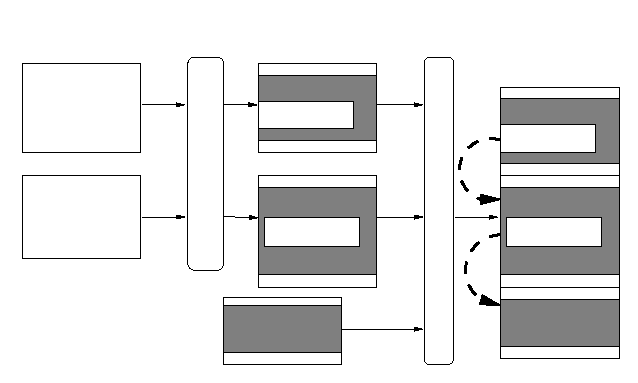
\includegraphics{img/tex/compilation_process}%
\end{picture}%
\setlength{\unitlength}{4144sp}%
%
\begingroup\makeatletter\ifx\SetFigFont\undefined%
\gdef\SetFigFont#1#2#3#4#5{%
  \reset@font\fontsize{#1}{#2pt}%
  \fontfamily{#3}\fontseries{#4}\fontshape{#5}%
  \selectfont}%
\fi\endgroup%
\begin{picture}(4602,2652)(46,-1918)
\put(766,-1771){\makebox(0,0)[lb]{\smash{\SetFigFont{10}{12.0}{\sfdefault}{\mddefault}{\updefault}{\color[rgb]{0,0,0}library}%
}}}
\put(181,-151){\makebox(0,0)[lb]{\smash{\SetFigFont{8}{9.6}{\sfdefault}{\mddefault}{\updefault}{\color[rgb]{0,0,0}\}}%
}}}
\put(181,-16){\makebox(0,0)[lb]{\smash{\SetFigFont{8}{9.6}{\sfdefault}{\mddefault}{\updefault}{\color[rgb]{0,0,0}\texttt{~~msg();}}%
}}}
\put(181,254){\makebox(0,0)[lb]{\smash{\SetFigFont{8}{9.6}{\sfdefault}{\mddefault}{\updefault}{\color[rgb]{0,0,0}\texttt{main()}}%
}}}
\put(181,119){\makebox(0,0)[lb]{\smash{\SetFigFont{8}{9.6}{\sfdefault}{\mddefault}{\updefault}{\color[rgb]{0,0,0}\texttt{\{}}%
}}}
\put(181,-1006){\makebox(0,0)[lb]{\smash{\SetFigFont{8}{9.6}{\sfdefault}{\mddefault}{\updefault}{\color[rgb]{0,0,0}\texttt{\}}}%
}}}
\put(181,-601){\makebox(0,0)[lb]{\smash{\SetFigFont{8}{9.6}{\sfdefault}{\mddefault}{\updefault}{\color[rgb]{0,0,0}\texttt{msg()}}%
}}}
\put(181,-871){\makebox(0,0)[lb]{\smash{\SetFigFont{8}{9.6}{\sfdefault}{\mddefault}{\updefault}{\color[rgb]{0,0,0}\texttt{~~puts();}}%
}}}
\put(181,-736){\makebox(0,0)[lb]{\smash{\SetFigFont{8}{9.6}{\sfdefault}{\mddefault}{\updefault}{\color[rgb]{0,0,0}\texttt{\{}}%
}}}
\put(361,-421){\makebox(0,0)[lb]{\smash{\SetFigFont{10}{12.0}{\sfdefault}{\mddefault}{\updefault}{\color[rgb]{0,0,0}util.c}%
}}}
\put(316,434){\makebox(0,0)[lb]{\smash{\SetFigFont{10}{12.0}{\sfdefault}{\mddefault}{\updefault}{\color[rgb]{0,0,0}main.c}%
}}}
\put( 46,614){\makebox(0,0)[lb]{\smash{\SetFigFont{10}{12.0}{\sfdefault}{\mddefault}{\updefault}{\color[rgb]{0,0,0}source code}%
}}}
\put(1801,614){\makebox(0,0)[lb]{\smash{\SetFigFont{10}{12.0}{\sfdefault}{\mddefault}{\updefault}{\color[rgb]{0,0,0}object files}%
}}}
\put(4006,434){\makebox(0,0)[lb]{\smash{\SetFigFont{10}{12.0}{\sfdefault}{\mddefault}{\updefault}{\color[rgb]{0,0,0}a.out}%
}}}
\put(3916,614){\makebox(0,0)[lb]{\smash{\SetFigFont{10}{12.0}{\sfdefault}{\mddefault}{\updefault}{\color[rgb]{0,0,0}program}%
}}}
\put(2116,479){\makebox(0,0)[lb]{\smash{\SetFigFont{10}{12.0}{\sfdefault}{\mddefault}{\updefault}{\color[rgb]{0,0,0}main.o}%
}}}
\put(3781,-16){\makebox(0,0)[lb]{\smash{\SetFigFont{10}{12.0}{\sfdefault}{\mddefault}{\updefault}{\color[rgb]{0,0,0}main}%
}}}
\put(3826,-691){\makebox(0,0)[lb]{\smash{\SetFigFont{10}{12.0}{\sfdefault}{\mddefault}{\updefault}{\color[rgb]{0,0,0}msg}%
}}}
\put(3781,-241){\makebox(0,0)[lb]{\smash{\SetFigFont{10}{12.0}{\sfdefault}{\mddefault}{\updefault}{\color[rgb]{0,0,0}msg}%
}}}
\put(1936,-61){\makebox(0,0)[lb]{\smash{\SetFigFont{10}{12.0}{\sfdefault}{\mddefault}{\updefault}{\color[rgb]{0,0,0}msg ??}%
}}}
\put(1936,164){\makebox(0,0)[lb]{\smash{\SetFigFont{10}{12.0}{\sfdefault}{\mddefault}{\updefault}{\color[rgb]{0,0,0}main}%
}}}
\put(2161,-421){\makebox(0,0)[lb]{\smash{\SetFigFont{10}{12.0}{\sfdefault}{\mddefault}{\updefault}{\color[rgb]{0,0,0}util.o}%
}}}
\put(1981,-691){\makebox(0,0)[lb]{\smash{\SetFigFont{10}{12.0}{\sfdefault}{\mddefault}{\updefault}{\color[rgb]{0,0,0}msg}%
}}}
\put(1981,-961){\makebox(0,0)[lb]{\smash{\SetFigFont{10}{12.0}{\sfdefault}{\mddefault}{\updefault}{\color[rgb]{0,0,0}puts ??}%
}}}
\put(1666,-1636){\makebox(0,0)[lb]{\smash{\SetFigFont{10}{12.0}{\sfdefault}{\mddefault}{\updefault}{\color[rgb]{0,0,0}puts}%
}}}
\put(766,-1591){\makebox(0,0)[lb]{\smash{\SetFigFont{10}{12.0}{\sfdefault}{\mddefault}{\updefault}{\color[rgb]{0,0,0}system}%
}}}
\put(3826,-961){\makebox(0,0)[lb]{\smash{\SetFigFont{10}{12.0}{\sfdefault}{\mddefault}{\updefault}{\color[rgb]{0,0,0}puts}%
}}}
\put(3781,-1591){\makebox(0,0)[lb]{\smash{\SetFigFont{10}{12.0}{\sfdefault}{\mddefault}{\updefault}{\color[rgb]{0,0,0}puts}%
}}}
\put(1531,-691){\rotatebox{90.0}{\makebox(0,0)[lb]{\smash{\SetFigFont{10}{12.0}{\sfdefault}{\mddefault}{\updefault}{\color[rgb]{0,0,0}compiler}%
}}}}
\put(3331,-916){\rotatebox{90.0}{\makebox(0,0)[lb]{\smash{\SetFigFont{10}{12.0}{\sfdefault}{\mddefault}{\updefault}{\color[rgb]{0,0,0}linker}%
}}}}
\end{picture}

\end{center}
\end{slide}

\begin{itemize}
\item Non-trivial programs are often split into several source code files that
contain related functions.  Such files can be compiled independently, and you
can even use different languages and different compilers for each file.  The
advantage is the speed of building, as only modified files are re-compiled (see
page \pageref{MAKE} on the \texttt{make} utility), and also flexibility, as you
can use some of the files in other programs as well.
\item The \emph{compiler} compiles each file into a corresponding object file.
Instead of external function pointers in the compiled code, the object file
contains a table of global symbols.
\item Then, the \emph{linker} combines the built object files and used
libraries into an output file.  By default, it also resolves all the references
to make sure all symbols used are available. 
\item Used code from the static libraries is copied to the executable file.
When using dynamic libraries, the executable only contains a list of them, the
linking process is then performed by the runtime linker (aka loader) on the
program execution.  For more on the dynamic linking process, see page
\pageref{RUNTIMELINKER}.
\item To select whether to use static or dynamic libraries, you use options for
the linker.  By default, dynamic libraries are used nowadays.  The source code
is same in either case.  There is also a mechanism (\texttt{dlopen},
\texttt{dlsym}\dots) that allows to load an additional dynamic library during
the program execution, and use it.  For more information, see page
\pageref{DLOPEN}.
\end{itemize}

%%%%%

\begin{slide}
\sltitle{Compilation of one file: preprocesor}
\begin{center}
\input{img/tex/preprocesor.pstex_t}
\end{center}
\end{slide}

\begin{itemize}
\item The preprocessor performs macro expansion, conditional compilation, and
inserts included files.  It also removes comments.
\item The preprocessor output can be provided via \texttt{cc -E} or calling
\texttt{cpp} directly.  However, some compilers have the preprocessor
functionality built in so calling the external preprocessor may not get the same
results.  You can of course use the preprocessor for anything else where its
functionality comes in handy, not just for C source code.
\item In a situation where you need to fix code full of includes and conditional
compilation, the output after the preprocessor phase may be very helpful to
locate the problem.
\item \texttt{cpp} (or \texttt{cc -E}) also allows you to see the whole tree of
included files, printed on the standard error output.  For that, use a separate
\texttt{-H} option (not \texttt{-EH}) and redirect the output to
\texttt{/dev/null}:

\begin{verbatim}
$ gcc -E -H tcp/connect.c >/dev/null
. /usr/include/stdio.h
.. /usr/include/sys/cdefs.h
... /usr/include/sys/_symbol_aliasing.h
... /usr/include/sys/_posix_availability.h
.. /usr/include/Availability.h
... /usr/include/AvailabilityInternal.h
.. /usr/include/_types.h
... /usr/include/sys/_types.h
.... /usr/include/machine/_types.h
..... /usr/include/i386/_types.h
etc...
\end{verbatim}

\item You cannot nest comments in C, so in order to temporarily disable code with
comments without deleting it, wrapping it in another comment will not work.
So, the preprocessor to your rescue -- use the conditional compilation feature:

\begin{verbatim}
...
#if 0
        /* some comment */
        some_function();
        /* another comment */
        another_function();
#endif
...
\end{verbatim}
\end{itemize}

%%%%%

\begin{slide}
\sltitle{Compilation of one file:  compiler}
\begin{center}
\begin{picture}(0,0)%
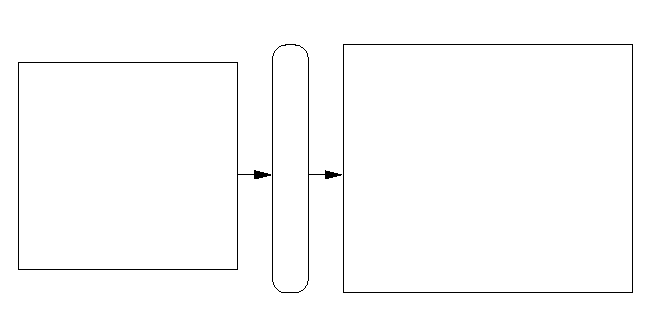
\includegraphics{img/tex/compiler}%
\end{picture}%
\setlength{\unitlength}{4144sp}%
%
\begingroup\makeatletter\ifx\SetFigFont\undefined%
\gdef\SetFigFont#1#2#3#4#5{%
  \reset@font\fontsize{#1}{#2pt}%
  \fontfamily{#3}\fontseries{#4}\fontshape{#5}%
  \selectfont}%
\fi\endgroup%
\begin{picture}(4704,2112)(-11,-1513)
\put(2566,209){\makebox(0,0)[lb]{\smash{\SetFigFont{10}{12.0}{\ttdefault}{\mddefault}{\updefault}{\color[rgb]{0,0,0}.globl main}%
}}}
\put(2566, 29){\makebox(0,0)[lb]{\smash{\SetFigFont{10}{12.0}{\ttdefault}{\mddefault}{\updefault}{\color[rgb]{0,0,0}~~~~.type main, @function}%
}}}
\put(2566,-121){\makebox(0,0)[lb]{\smash{\SetFigFont{10}{12.0}{\ttdefault}{\mddefault}{\updefault}{\color[rgb]{0,0,0}main:}%
}}}
\put(2566,-286){\makebox(0,0)[lb]{\smash{\SetFigFont{10}{12.0}{\ttdefault}{\mddefault}{\updefault}{\color[rgb]{0,0,0}~~~~pushhl \%ebp}%
}}}
\put(2566,-451){\makebox(0,0)[lb]{\smash{\SetFigFont{10}{12.0}{\ttdefault}{\mddefault}{\updefault}{\color[rgb]{0,0,0}~~~~movl \%esp, \%ebp}%
}}}
\put(2566,-616){\makebox(0,0)[lb]{\smash{\SetFigFont{10}{12.0}{\ttdefault}{\mddefault}{\updefault}{\color[rgb]{0,0,0}~~~~pushl \$.LC0}%
}}}
\put(2566,-781){\makebox(0,0)[lb]{\smash{\SetFigFont{10}{12.0}{\ttdefault}{\mddefault}{\updefault}{\color[rgb]{0,0,0}~~~~call puts}%
}}}
\put(2566,-946){\makebox(0,0)[lb]{\smash{\SetFigFont{10}{12.0}{\ttdefault}{\mddefault}{\updefault}{\color[rgb]{0,0,0}~~~~addl \$4, \%esp}%
}}}
\put(2566,-1111){\makebox(0,0)[lb]{\smash{\SetFigFont{10}{12.0}{\ttdefault}{\mddefault}{\updefault}{\color[rgb]{0,0,0}.L1:}%
}}}
\put(2566,-1276){\makebox(0,0)[lb]{\smash{\SetFigFont{10}{12.0}{\ttdefault}{\mddefault}{\updefault}{\color[rgb]{0,0,0}~~~~leave}%
}}}
\put(2566,-1441){\makebox(0,0)[lb]{\smash{\SetFigFont{10}{12.0}{\ttdefault}{\mddefault}{\updefault}{\color[rgb]{0,0,0}~~~~ret}%
}}}
\put(2116,-916){\rotatebox{90.0}{\makebox(0,0)[lb]{\smash{\SetFigFont{10}{12.0}{\sfdefault}{\mddefault}{\updefault}{\color[rgb]{0,0,0}compiler}%
}}}}
\put(3331,479){\makebox(0,0)[lb]{\smash{\SetFigFont{10}{12.0}{\sfdefault}{\mddefault}{\updefault}{\color[rgb]{0,0,0}main.s}%
}}}
\put(136, 29){\makebox(0,0)[lb]{\smash{\SetFigFont{10}{12.0}{\ttdefault}{\mddefault}{\updefault}{\color[rgb]{0,0,0}int puts(char *s);}%
}}}
\put(136,-331){\makebox(0,0)[lb]{\smash{\SetFigFont{10}{12.0}{\ttdefault}{\mddefault}{\updefault}{\color[rgb]{0,0,0}extern int var\_{}a;}%
}}}
\put(136,-691){\makebox(0,0)[lb]{\smash{\SetFigFont{10}{12.0}{\ttdefault}{\mddefault}{\updefault}{\color[rgb]{0,0,0}main()}%
}}}
\put(136,-871){\makebox(0,0)[lb]{\smash{\SetFigFont{10}{12.0}{\ttdefault}{\mddefault}{\updefault}{\color[rgb]{0,0,0}\{}%
}}}
\put(136,-1051){\makebox(0,0)[lb]{\smash{\SetFigFont{10}{12.0}{\ttdefault}{\mddefault}{\updefault}{\color[rgb]{0,0,0}~~puts("hello");}%
}}}
\put(136,-1231){\makebox(0,0)[lb]{\smash{\SetFigFont{10}{12.0}{\ttdefault}{\mddefault}{\updefault}{\color[rgb]{0,0,0}\}}%
}}}
\put(586,344){\makebox(0,0)[lb]{\smash{\SetFigFont{10}{12.0}{\sfdefault}{\mddefault}{\updefault}{\color[rgb]{0,0,0}main.i}%
}}}
\end{picture}

\end{center}
\end{slide}

\begin{itemize}
\item The picture is an example output for the x86 platform, 32-bit, with AT\&T
syntax.
\item Compilation from the C language into assembler.
\item The assembler output file is the result of \texttt{cc -S}.
\end{itemize}

%%%%%

\begin{slide}
\sltitle{Compilation of one file: assembler}
\begin{center}
\input{img/tex/assembler.pstex_t}
\end{center}
\end{slide}

\begin{itemize}
\item Again an example for the x86 platform, 32-bit.
\item Compilation from the assembler language into the object code.
\item The output file is the result of \texttt{cc -c}.
\end{itemize}

%%%%%

\begin{slide}
\sltitle{Compiler}
\renewcommand{\arraystretch}{1.1}
\begin{itemize}
\item usage:\\
\texttt{cc [\emph{options}] \emph{file} \dots}
\item the most important options:\\
\begin{tabular}{ll}
\texttt{-o \emph{file}} & output file name\\
\texttt{-c} & only compile, do not link\\
\texttt{-E} & only preprocessor\\ 
\texttt{-l} & link with the specified library\\
\texttt{-L\emph{directory}} & add a directory to search when using \texttt{-l}\\
\texttt{-O\emph{level}} & optimization level\\
\texttt{-g} & compile with debug information\\
\texttt{-D\emph{name}} & define a macro for the preprocessor\\
\texttt{-I\emph{directory}} & add a directory to search for \texttt{\#include} files
\end{tabular}
\end{itemize}
\end{slide}

\begin{itemize}
\item \texttt{-l}/\texttt{-L} are actually options for the linker, ie. the
compiler will pass them on onto the linker.
\item Both the compiler and linker have an extensive list of additional options
that influence the generated code and what warnings are printed during the
compilation/linking based on the chosen language and the standard.  See manual
pages for \texttt{cc}, \texttt{gcc}, and/or \texttt{ld}.
\end{itemize}

%%%%%

\pdfbookmark[1]{standard macros}{stdmacros}

\begin{slide}
\sltitle{UNIX standard macros}
\begin{tabbing}
\hskip 13em \= \kill
\verb#__FILE__#, \verb#__LINE__#,\\\verb#__DATE__#, \verb#__TIME__#,\\
\verb#__cplusplus#, etc.
\> are standard macros for the compiler \\\>C/C++\\
\verb#unix# \> always defined if on Unix\\
\verb#mips#, \verb#i386#, \verb#sparc# \> hardware architecture\\
\verb#linux#, \verb#__APPLE__#, \verb#sun#, \verb#bsd# \> operating system\\
\verb#_POSIX_SOURCE#,\\\verb#_XOPEN_SOURCE#
\> build using the specific standard\\
\end{tabbing}
\end{slide}

\begin{slide}
\sltitle{UNIX standard macros (cont.)}

To build using a specific standard, you need to define one of the macros below
before any \verb.#include..  Then include \texttt{unistd.h}.

\vspace{2ex}

\begin{tabular}{l@{\hspace{3em}}l}
\emsl{UNIX 98} &\verb.#define _XOPEN_SOURCE 500.\\
\emsl{SUSv3} &\verb.#define _XOPEN_SOURCE 600.\\
\emsl{SUSv4} &\verb.#define _XOPEN_SOURCE 700.\\
\emsl{POSIX1990} &\verb.#define _POSIX_SOURCE.
\end{tabular}
\end{slide}

\begin{itemize}
\item The way it works is that you use specific macros to define what you
want (eg. \texttt{\_POSIX\_SOURCE}), and then you use other macros (eg.
\texttt{\_POSIX\_VERSION}) to find out what you actually got.  You always have
to include \texttt{unistd.h} after you set the macros and use a compiler that
supports what you want.  For example, below we tried to compile
\example{basic-utils/standards.c} which requires SUSv3, on a system supporting
SUSv3 (Solaris 10), using a compiler that only supports SUSv2 (the compiler
defined in SUSv3 is \texttt{c99}).  Note that the default behavior of your
compiler might be same as \texttt{c89}.

\begin{verbatim}
$ cat standards.c 
#define _XOPEN_SOURCE   600
/* you must #include at least one header !!! */
#include <stdio.h>
int main(void)
{
        return (0);
}
$ c89 basic-utils/standards.c 
"/usr/include/sys/feature_tests.h", line 336: #error: "Compiler or
options invalid; UNIX 03 and POSIX.1-2001 applications require
the use of c99"
cc: acomp failed for standards.c
\end{verbatim}
%\item the source of macros for standard can be mentioned already on page
%\pageref{UNIXSTANDARDS}. Mentioned header file \texttt{feature\_tests.h}
%on Solaris
\item See the documentation for your compiler about what other macros can be
used.
\item See page \pageref{C_LANGUAGE} for more information on standards.
\item Regarding macros for specific standards, you can find very good
information in chapter 1.5 in [Rochkind]. See also
\example{basic-utils/suvreq.c}.

\begin{verbatim}
int
main(void)
{
#ifdef unix
        printf("Yeah!\n");
#else
        printf("Oh, no.\n");
#endif
        return (0);
}
\end{verbatim}
\item For an example on using \texttt{\_\_LINE\_\_}, see
\example{basic-utils/main\_\_LINE\_\_.c}
\end{itemize}

%%%%%

\pdfbookmark[1]{link editor}{linker}

\begin{slide}
\sltitle{Link editor (linker)}
\begin{itemize}
\item Invocation:\\
\texttt{ld [\emph{options}] \emph{file} \dots}\\
\texttt{cc [\emph{options}] \emph{file} \dots}
\item Often used options:\\
\begin{tabular}{ll}
\texttt{-o \emph{file}} & output file name (default \texttt{a.out})\\
\texttt{-l\emph{lib}} & link with library \texttt{lib\emph{lib}.so} or
\texttt{lib\emph{lib}.a}\\ 
\texttt{-L\emph{path}} & path to libraries (\texttt{-l\emph{lib}})\\
\texttt{-shared} & create a dynamic library\\
\texttt{-non\_shared} & create a static executable
\end{tabular}
\end{itemize}
\end{slide}

\begin{itemize}
\item A linker takes one or more objects generated by a compiler and creates a
binary executable, library, or another object file suitable for another linking
phase.
\item Note that different systems support different options.  For example,
\texttt{ld} on Solaris does not support \texttt{-shared} and
\texttt{-non\_shared}, and you have to use alternatives.
\item An option \texttt{-R} allows to specify where to look for libraries when
loading the executable via the dynamic linker.  That path might be different
from the path used during building the object, modifiable via \texttt{-L}.
\item Often you do not use the linker directly at all but pass all the linker
options via the compiler.
\end{itemize}

%%%%%

\pdfbookmark[1]{make}{make}

\begin{slide}
\sltitle{Maintaining programs (\texttt{make})}
\renewcommand{\baselinestretch}{1}
\begin{itemize}
\item \emsl{source code}\\
\begin{minipage}[t]{3.3cm}
main.c\\
\setbox0=\hbox{\begin{minipage}[t]{3.1cm}
\begin{verbatim}
#include "util.h"
main()
{
  msg();
}
\end{verbatim}
\end{minipage}}
\framebox{\box0}
\end{minipage}\hfill
\begin{minipage}[t]{2.2cm}
util.h\\
\setbox1=\hbox{\begin{minipage}[t]{2cm}
\begin{verbatim}
void msg();
\end{verbatim}
\end{minipage}}
\framebox{\vphantom{\texttt{\#include"}}\box1}
\end{minipage}\hfill
\begin{minipage}[t]{3.3cm}
util.c\\
\setbox0=\hbox{\begin{minipage}[t]{3.2cm}
\begin{verbatim}
#include "util.h"
msg()
{
  puts();
}
\end{verbatim}
\end{minipage}}
\framebox{\box0}
\end{minipage}
\end{itemize}
\begin{minipage}[t]{3.7cm}
\begin{itemize}
\item \emsl{dependencies}\\\vskip-1ex
\renewcommand{\arraystretch}{0.1}
\setlength{\tabcolsep}{0.25ex}
\begin{tabular}{lclcl}
\texttt{main.c} &            &                 &            & \\
                & $\searrow$ &                 &            & \\
		&            & \texttt{main.o} &            & \\
		& $\nearrow$ &                 & $\searrow$ & \\
\texttt{util.h} &            &                 &            & \texttt{prog} \\
                & $\searrow$ &                 & $\nearrow$ & \\
		&            & \texttt{util.o} &            & \\
		& $\nearrow$ &                 &            & \\
\texttt{util.c} &            &                 &            & \\
\end{tabular}
\end{itemize}
\end{minipage}\hfill
\begin{minipage}[t]{6.5cm}
\begin{itemize}
\item \emsl{file} \texttt{Makefile}\\
\setbox0=\hbox{\begin{minipage}[t]{5.9cm}
\begin{verbatim}
prog : main.o util.o
        cc -o prog main.o util.o
main.o : main.c util.h
        cc -c main.c
util.o : util.c util.h
        cc -c util.c
\end{verbatim}
\end{minipage}}
\framebox{\box0}
\end{itemize}
\end{minipage}
\end{slide}

\label{MAKE}.

\begin{itemize}
\item You could compile and link the program via one invocation of a compiler,
or write a simple shell script.  However, by using \texttt{make} you will only
update a target if its dependencies have been modified.  In other words, a well
written makefile will cause to re-compile only what is really necessary after
some files have been changed.  You could always do something like
``\texttt{make clean; make all}'' but if the whole compilation process takes
minutes or even hours, you really want a well written \texttt{Makefile}.
\item A line ``\verb#prog : main.o util.o#'' defines that before \texttt{prog}
is checked, the existence of
\texttt{main.o} and \texttt{util.o} needs to be checked, and also whether they
are up to date.  That check is performed recursively.  After that, the existence
of \texttt{prog} is checked and whether it is up-to-date, which means whether
the last modification time is younger than that of \texttt{main.o} and
\texttt{util.o}.  If yes, nothing else is done.  If not, the command on the next
line is performed.
\item \texttt{make} is usually run with an argument specifying the target to be
built; if run without arguments, the first target in the \texttt{Makefile} is
used.  That often is \texttt{all} which if the standard Unix convention is
followed, builds everything that can be built.  After that, \texttt{make
install} often follows, etc.
\item \texttt{make} is a universal tool, useful not just for building source
code.  For example, to build this material from various \LaTeX{} and other source
files, \texttt{make} is used as well.
\item Example: \example{basic-utils/Makefile01}.  Note that if a non-standard
make file is used, you need the \texttt{-f} option: ``\texttt{make -f
Makefile01}''.
\end{itemize}

%%%%%

\begin{slide}
\sltitle{Syntax of the \texttt{make} input file}
\begin{itemize}
\item \makebox[4cm][l]{target dependencies:}
\texttt{\emph{targets} : [\emph{files}]}
\item \makebox[4cm][l]{commands to be executed:} \verb#<Tab>#\texttt{\emph{command}}
\item \makebox[4cm][l]{comment:} \texttt{\#\emph{comment}}
\item \makebox[4cm][l]{line continuation:}
\texttt{\emph{line-begin}}\verb#\#\\
\makebox[4cm][l]{~} \texttt{\emph{line-continuation}}
\end{itemize}
\end{slide}

\begin{itemize}
\item \emsl{Note that the line with a command starts with a tab, not
spaces.}  Every command line is executed via its own shell invocation.  If
multiple commands need to be executed via the same shell process, all but the
last line needs to be terminated with a backslash.  See the following example
where the last two \texttt{echo} commands are part of the same \texttt{if}
construct.

\begin{verbatim}
$ cat basic-utils/Makefile02
all:
        @echo $$$$
        @echo $$$$
        @if true; then \
                echo $$$$; \
                echo $$$$; \
        fi
$ make -f Makefile02
5513
5514
5515
5515
\end{verbatim}

\item The backslash works as a word separator and a space is inserted.  See
the following example: \example{basic-utils/Makefile07}.
\item Using a double \texttt{\$} suppresses the special meaning of a dollar
sign, see the next slide.
\item A character \texttt{@} at the beginning of a line suppresses its printout.
Otherwise, \texttt{make} always prints out what is gonna be executed next.
\item For a dry run, ie. to see what would be executed, but do not execute
anything, use option \texttt{-n}.
\item A character \texttt{-} at the beginning of a line causes \texttt{make} to
ignore a non-zero return value (usually indicating a failure), otherwise
\texttt{make} reports the error and bails out right away.  Example:
\example{basic-utils/Makefile04}.
\item 
\begin{verbatim}
test1:
        false
        echo "OK"

test2:
        -false
        echo "OK"
\end{verbatim}
\end{itemize}

%%%%%

\begin{slide}
\sltitle{Macros (\texttt{make})}
\begin{itemize}
\item macro definition:\\
\hspace*{5em}\texttt{name = string}
\item continuation via a backslash inserts a space
\item undefined macros are empty
\item ordering of macro definitions is not important
\item defining a macro on a command line: \\
\hspace*{5em}\texttt{make \emph{target} \emph{name}=\emph{string}}
\item macro invocation: \\
\hspace*{5em}\texttt{\$\emph{name}} (only one character
\texttt{\emph{name}}), \\
\hspace*{5em}\texttt{\$\{\emph{name}\}} or \texttt{\$(\emph{name})}
\item environment variables are accessible as macros (eg. \texttt{\$\{EDITOR\}})
\end{itemize}
\end{slide}

\begin{itemize}
\item If a macro is defined multiple times, the last definition rules, you can
see an example in \example{basic-utils/Makefile03}.
\item You cannot define a macro recursively, see
\example{basic-utils/Makefile05}:

\begin{alltt}
\$ cat basic-utils/Makefile05
M=value1
M=\$(M) value2
all:
        echo \$(M)
\$ make -f Makefile05
Variable M is recursive.
\end{alltt}
\item Often extended \texttt{make} versions are used, eg. GNU (\texttt{gmake})
or BSD.
\item To write a non-trivial \texttt{Makefile} that will work with
different \texttt{make} implementations is not a simple task.  Therefore
projects as GNU Automake exist.  For a simple conditional compilation, where
based on the system we need to set different options, the following code might
come in handy.  A character ` is a back quote, and a ' is a normal single quote:

\begin{verbatim}
CFLAGS=`x=\`uname\`; \
        if [ $${x} = FreeBSD ]; then \
                echo '-Wall'; \
        elif [ $${x} = SunOS ]; then \
                echo '-v'; \
        elif [ $${x} = Linux ]; then \
                echo '-Wall -g'; \
        fi`

all:
        @echo "$(CFLAGS)"
\end{verbatim}

\item In other situations it is recommended or even needed to use utilities like
\texttt{autoconf} or \texttt{automake}.
\item Some \texttt{make} implementations support directives for conditional
processing, eg.  BSD make.  Example: \example{basic-utils/Makefile08.bsd}.
\item With the \texttt{-e} option, we can force \texttt{make} to ignore a
variable definition in the input file if an environment variable of the same
name exists.  By default \texttt{make} accepts environment variables only if
they are not defined in the input file.  Example:
\example{basic-utils/Makefile06}.
\item In general, \texttt{make} is a immensely powerful tool, just take a look
at system make files of any Unix-like system.  A typical feature of such build
systems is that there is no documentation on how it works internally so you have
to dig in deep if you need to understand or modify it -- and that usually is not
for the faint-hearted.
\end{itemize}

%%%%%

\pdfbookmark[1]{dynamic linker}{ldso}

\begin{slide}
\sltitle{Dynamic linker (loader)}

\begin{itemize}
\item the compilation phase requires all needed dynamic libraries to check
accessibility of used symbols
\item \emsl{loading external shared libraries into a running process happens on
program execution}. That is what a \emsl{dynamic linker} does  (\emph{run-time
linker}, \emph{loader}).
\item list of required dynamic libraries is in the \texttt{.dynamic} section of
an ELF object
\item system by default looks for shared libs in certain locations
\item located libraries are mapped to the process address space via
\funnm{mmap}() (will be later)
\end{itemize}
\end{slide}

\label{RUNTIMELINKER}

\begin{itemize}
\item An ELF object format is explained on page \pageref{ELF}.
\item In the ELF \texttt{.dynamic} section, you can add additional paths to
search for the libraries using tags \texttt{RUNPATH}/\texttt{RPATH}.
\item The process of an execution of a dynamically linked program works like
this:
\begin{itemize}
\item The kernel in \texttt{exec()} maps the program to a newly created process
address space and finds out what a dynamic linker is used (see \texttt{.interp}
below).
\item The kernel maps the dynamic linker to the process address space as well
and calls the linker's \texttt{main()} function.  As a dynamic linker is an
executable program by itself, it has \texttt{main()}.  You can usually also run
a dynamic linker on a command line if you want to, that is mostly useful for
debugging and experimenting with a dynamic linker.
\item The linker gets the list of required libraries from the program ELF header,
maps those libraries to the process address space, and calls their initialization
functions if those exist.  All dependencies not set as 
\emph{lazy} (see page \pageref{DLOPEN}) are mapped recursively via breadth
search.
\item The linker's job is done at that point and calls the program
\texttt{main()} function.
\item A process may continue to use the dynamic linker during program execution
via calls like \texttt{dlopen()} etc.  See page \pageref{DLOPEN} for more
information.
\end{itemize}
\item Note that the dynamic linker does not run as a separate process (unless
you run it like that) even though it has its own \texttt{main()} function.  It is
used within an address space of an executed program.  The program, dynamic
linker, and dynamic libraries constitute a single process.

\item The following examples \emsl{are from Solaris}.  Finding equivalent
commands and/or options on Linux is left as an exercise to the reader.
\begin{itemize}
\item ELF sections are listed via \texttt{elfdump -c} (GNU has
\texttt{objdump} and \texttt{readelf}).  More on program sections on page
\pageref{ELF}.
\item What a dynamic linker is used is in section \texttt{.interp}, see
''\texttt{elf\-dump -i}'' and ``\texttt{ld -I}''.  It means you could write your
own dynamic linker and set it via the \texttt{-I} option for \texttt{ld} to your
program.  Needless to say, such an enterprise would not be an easy feat at
all.
\item To list the dynamic section, use \texttt{elfdump -d}, dynamic libraries
are set as \texttt{NEEDED}.
\item Finding out shared object dependencies is very easy via the
\texttt{ldd} command (Solaris, Linux, BSD).  It displays paths to the specific
libraries (ie. full paths) that will be used if the program is run in the
same environment (see right below for more information).  The command resolves
the dependencies recursively so you will also see dynamic libraries that are used
by other libraries and not directly by the program.  To find out what exactly
depends on what, use the \texttt{-v} option.  macOS does not have \texttt{ldd},
use \texttt{otool -L} instead.
\item What libraries are eventually used when running the program could be
different from what \texttt{ldd} shows.  For example, 
one could use the \texttt{LD\_PRELOAD} mechanism.  For that reason,
Solaris has a \texttt{pldd} command which provides the library dependencies for
a running process.  For an example on \texttt{LD\_PRELOAD} with \texttt{gcc}:
use already mentioned \texttt{Ma\-ke\-file01}, and compile
\example{basic-utils/preload.c} like this:
\begin{verbatim}
gcc -shared -o libpreload.so preload.c
\end{verbatim}
Run the program then which interposes a system
call \texttt{close()} like this:
\begin{verbatim}
LD_PRELOAD=./libpreload.so ./a.out
\end{verbatim}
\item Most of the information listed here can be found in the manual page for the
Solaris dynamic linker, \texttt{ld.so.1(1)}, and much more in the excellent
\emph{Linkers and Libraries Guide} on \texttt{docs.oracle.com}.  If you use
FreeBSD, its dynamic linker is \texttt{ld-elf.so.1}, on Linux distros it is
usually \texttt{ld-linux.so.1}, it is \texttt{rld} on SGI IRIX etc.
\item You can also configure the dynamic linker via setting environment
variables.  For example, try this on Solaris:
\begin{verbatim}
LD_LIBRARY_PATH=/tmp LD_DEBUG=libs,detail date
\end{verbatim}
and to find out what options you have to debug the dynamic linker there:
\begin{verbatim}
LD_DEBUG=help date
\end{verbatim}
\item To tell the linker to also look for dynamic libraries in directories other
than the default ones (paths from \texttt{LD\_LIBRARY\_PA\-TH} are searched
first), use it like the following:
\begin{verbatim}
$ cp /lib/libc.so.1 /tmp
$ LD_LIBRARY_PATH=/tmp sleep 100 &
[1] 104547
$ pldd 104547
104547: sleep 100
/tmp/libc.so.1
/usr/lib/locale/cs_CZ.ISO8859-2/cs_CZ.ISO8859-2.so.3
\end{verbatim}
\item You can also edit ELF objects via \texttt{elfedit(1)} on Solaris.  You can
change \texttt{RUNPATH}, for example.
\end{itemize}
\item \label{EVIL_LDLIBPATH} In general, you should not use
\texttt{LD\_LIBRARY\_PATH} for anything else than debugging during the
development or when moving libraries between directories.  You can find lots of
articles on ``why is \texttt{LD\_LIBRARY\_PATH} evil?'' etc.  For example,
\url{http://xahlee.org/UnixResource\_dir/\_/ldpath.html}.

\par
This variable is often misused in the start-up scripts because the command(s)
is/are incorrectly linked and the dynamic linker would not otherwise find the
correct libraries.  The typical side effect, however, is that the program(s)
subsequently start(s) additional programs that use the same libraries but as all
children inherit the environment, those programs are forced to use libraries
from non-default directories, and possibly those contain libraries of different
versions from those that the programs were initially built with.  Quite often
this might be hard to find when something goes bad and you start seeing
unexpected behavior.  Commands like \texttt{pldd} come in handy in such
situations.
\end{itemize}

%%%%%

\pdfbookmark[1]{API/ABI}{APIABI}

\begin{slide}
\sltitle{API vs ABI}

API -- Application Programming Interface

\begin{itemize}
\item interface used in the \emsl{source code} to use another software
component like a library, OS kernel, or your own code -- eg.
\texttt{exit(1)}, \texttt{printf("hello\bs{}n")} or \texttt{my\_function(1,
2)}
\item \dots{}so that the same source code could be compiled on all systems
supporting a given API
\end{itemize}

ABI -- Application Binary Interface

\begin{itemize}
\item low-level binary interface between \emsl{modules} (eg.  \texttt{a.out}
and \texttt{libc.so.1} or even \texttt{a.out} and \texttt{a.out})
\item \dots{}so that the built module could be used wherever the same ABI is
supported
\end{itemize}
\end{slide}

\label{API_ABI}

\begin{itemize}
\item In short -- an API is source code based while an ABI is binary based.
\item An example of an API is one defined by the POSIX.1 standard or the set of
system calls for a given system.
\item An example of an ABI is the System V AMD64 ABI, followed on Solaris,
Linux, FreeBSD, macOS, and other systems.
\item ABI defines the calling convention interface to the called machine code, eg.
how parameters are passed (pushed on the stack, placed in registers, or a mix
of both) or how return value is returned.
\item API defines a set of functions, its parameters and their types, and
function return values.  The API may also include global variables --
\texttt{errno}, for example.
\item The following example represents what happens if a library ABI is changed
and the new library replaces the old one.  Note that the dynamic linker cannot
detect that the function symbol did not change.  The given change is also an
API change and the problem would be fixed if \texttt{main.c} was recompiled
with the correct prototype for function \texttt{my\_add}.  However,
recompiling is often not desirable as one might end up recompiling the whole
system.  That is why keeping backward compatibility for library ABI is so
important.

The first result is expected, ie. \texttt{3}:

\begin{verbatim}
$ cat main.c 
#include <stdio.h>

int my_add(int a, int b);

int
main(void)
{
        (void) printf("%d\n", my_add(1, 2));
        return (0);
}

$ cat add.c
int
my_add(int a, int b)
{
        return (a + b);
}

$ gcc -shared -o libadd.so add.c
$ gcc -L. -ladd -Xlinker -R . main.c
$ ./a.out 
3
\end{verbatim}

Now imagine a new library came, one with a modified ABI in function
\texttt{my\_add}.  Note that we replaced the old library with the new one.
Now, instead of 4 byte integers, 64-bit longs are used.  When you run the
program again, you will get an incorrect return value:

\begin{verbatim}
$ cat add2.c
int64_t
my_add(int64_t a, int64_t b)
{
        return (a + b);
}

$ gcc -shared -o libadd.so add2.c 
$ ./a.out 
-1077941135
\end{verbatim}

\item \label{ABI_MAIN} Example: \example{lib-abi/abi-main.c} (see the block
comment in the file on how to use other files located in the same directory).
\item To change an ABI safely, you need library versioning -- if the library
ABI change is not backward compatible, a bumped up version needs to prevent
running the program without rebuilding it.   However, in that case you need to keep
the old library on the system.  Note that having different versions of the same
library might become a problem by itself, for example if more versions of such
a library get loaded into the program address space.
\item The way versioning works in ELF (see page \pageref{ELF}) is that the
library file name incorporates a version.  The \texttt{SONAME} in the dynamic
section then lists the full name of the library, including the version.  When
the loader searches for the libraries, it searches for the filename from the
\texttt{SONAME} field.
\item Example of what exact libraries and their versions are needed for the
Secure shell client on a Linux distribution.  You see that, for example, the
OpenSSL library version used by the SSH client is 1.0.0.:

\begin{verbatim}
$ readelf -d /usr/bin/ssh

Dynamic section at offset 0xb0280 contains 34 entries:
  Tag        Type           Name/Value
0x0000000000000001 (NEEDED) Shared library: [libsctp.so.1]
0x0000000000000001 (NEEDED) Shared library: [libcrypto.so.1.0.0]
0x0000000000000001 (NEEDED) Shared library: [libdl.so.2]
0x0000000000000001 (NEEDED) Shared library: [libz.so.1]
0x0000000000000001 (NEEDED) Shared library: [libresolv.so.2]
0x0000000000000001 (NEEDED) Shared library: [libpthread.so.0]
0x0000000000000001 (NEEDED) Shared library: [libgssapi.so.3]
0x0000000000000001 (NEEDED) Shared library: [libc.so.6]

$ openssl version
OpenSSL 1.0.2n  7 Dec 2017

$ ls /usr/lib/libcrypto.so.1.0.0
/usr/lib/libcrypto.so.1.0.0
\end{verbatim}

\par The OpenSSL library version is kept 1.0.0 even though the real version is
actually 1.0.2n.  That is because the micro versions (``z'' in x.y.z) do not
change the ABI binary compatibility (change in ``y'' does).  So, such a number
must not be in the \texttt{SONAME} field otherwise you would need rebuilt
binaries that depend on OpenSSL, even on a binary compatible micro upgrade.
\end{itemize}

%%%%%

\begin{slide}
\sltitle{Debugger \texttt{dbx}}
\begin{itemize}
\item Usage:\\
\texttt{dbx [ \emph{options} ] [ \emph{program} [ \emph{core} ] ]}
\item Most common commands:\\
\renewcommand{\arraystretch}{0.9}
\begin{tabular}{ll}
\texttt{run [\emph{arglist}]} & program start\\
\texttt{where} & print stack\\
\texttt{print \emph{expr}} & print expression\\
\texttt{set \emph{var} = \emph{expr}} & change value of variable\\
\texttt{cont} & continue program run\\
\texttt{next}, \texttt{step} & execute a line (with/out going into func)\\
\texttt{stop \emph{condition}} & set breakpoint\\
\texttt{trace \emph{condition}} & remove tracepoint\\
\texttt{command \emph{n}} & action on breakpoint (commands follow)\\
\texttt{help [\emph{name}]} & help\\
\texttt{quit} & debugger exit
\end{tabular}
\end{itemize}
\end{slide}

\begin{itemize}
\item Basic line oriented debugger with symbols; to fully use it, the program to
be debugged has to be compiled with debugging data (\texttt{cc -g}). The program
is then started from debugger using the \texttt{run} command, or the debugger
can be connected to an already running process. \texttt{dbx} can also be used to
analyze program crashes, provided a \texttt{core} file was generated.
\item It is possible to find it e.g. on Solaris, it is not present by default
on other systems.
\item For source line debugging it is not necessary to use just the \texttt{-g}
option for translation, it is also necessary to have the object files and source
files available in the same location as they were used for compilation.
This is typically true when debugging on the system where the code is written.
For other use cases it is necessary to provide the needed files, the dbx
command \texttt{pathmap} can help with that.
\item \texttt{gdb}-compatible mode can be enabled using \texttt{gdb on}.
If you want to know the \texttt{dbx} equivalent command to concrete
\texttt{gdb} command, see the \texttt{help FAQ}; the very first question is
``A.1  Gdb does $<$something$>$; how do I do it in dbx?''
\item If the option \texttt{-g} is not used, dbx will be still usable on
Solaris, because it will print function arguments. On BSD systems and Linux
distributions, the \texttt{-g} has to be used, otherwise the debuggers will not
be of much use. This is demonstrated in the \example{debug/dbx.c} example.
When compiling with gcc and using gdb the \texttt{where} command will not show
the function parameters, while on Solaris with the Studio compiler and dbx
debugger, the function parameters will be shown.
\item Example: \example{debug/coredump.c}. After compilation and running the
program will crash and a core dump will be generated (if permitted on the system;
also see \texttt{ulimit -c})

\begin{verbatim}
$ cc coredump.c
$ ./a.out 
Segmentation Fault (core dumped)
$ dbx ./a.out core
Reading a.out
core file header read successfully
Reading ld.so.1
Reading libc.so.1
program terminated by signal SEGV (no mapping at the fault address)
0x08050a05: bad_memory_access+0x0015:   movb     %al,0x00000000(%edx)
(dbx) where                                                                  
=>[1] bad_memory_access(0x8047ae8, 0x8047a44, ...
  [2] main(0x1, 0x8047a50, 0x8047a58, 0x8047a0c), at 0x8050a1b 
\end{verbatim}

Based on the above it is possible to say in which function the program crashed.
What we cannot see is the exact line in the code. For that, the program has to be
compiled with debugging symbols, i.e. ``\texttt{cc -g coredump.c}''.

\begin{verbatim}
$ cc -g coredump.c
$ dbx ./a.out core
Reading a.out
core file header read successfully
Reading ld.so.1
Reading libc.so.1
program terminated by signal SEGV (no mapping at the fault address)
Current function is bad_memory_access
    8           x[0] = '\0';
(dbx) 
\end{verbatim}

\end{itemize}

%%%%%

\begin{slide}
\sltitle{GNU debugger \texttt{gdb}}
\begin{itemize}
\item Usage:\\
\texttt{gdb [ \emph{options} ] [ \emph{program} [ \emph{core} ] ]}
\item Most common commands:\\
\renewcommand{\arraystretch}{0.9}
\begin{tabular}{ll}
\texttt{run [\emph{arglist}]} & program start\\
\texttt{bt} & print stack\\
\texttt{print \emph{expr}} & print expression\\
\texttt{set \emph{var} = \emph{expr}} & change value of variable\\
\texttt{cont} & continue program run\\
\texttt{next}, \texttt{step} & execute a line (with/out going into func)\\
\texttt{break \emph{condition}} & set breakpoint\\
\texttt{help [\emph{name}]} & print help\\
\texttt{quit} & debugger exit
\end{tabular}
\end{itemize}
\end{slide}

\begin{itemize}
\item GNU analogy of \texttt{dbx}. The \texttt{dbx} compatibility mode can be
enabled using the \texttt{-dbx} option.
\item Most platforms today offer debuggers with a graphical front end. Often they
are implemented on top of \texttt{gdb}.

\item \begin{verbatim}
#include <stdio.h>
int main(void) {
  printf("hello, world\n");
  return (0);
}
$ cc -g main.c 
$ gdb -q a.out
(gdb) break main
Breakpoint 1 at 0x8048548: file main.c, line 4.
(gdb) run
Starting program: /share/home/jp/src/gdb/a.out 

Breakpoint 1, main () at main.c:4
4         printf("hello, world\n");
(gdb) next
hello, world
5         return (0);
(gdb) c
Continuing.
Program exited normally.
(gdb) q
\end{verbatim}
\item Debuggers are a great help when your program exits with a
``segmentation error'' -- i.e. when accessing memory incorrectly.
When the \texttt{-g} option is used during compilation, the debugger will be able to
show exact line of code where the problem happened.
Concrete example (can you tell why the program behaves in such a way?):
\begin{verbatim}
$ cat -n main.c
     1  int
     2  main(void)
     3  {
     4          char *c = "hey world";
     5          c[0] = '\0';
     6          return (0);
     7  }
}
$ gcc -g main.c
$ ./a.out
Bus error (core dumped)
$ gdb a.out a.out.core
...
Core was generated by `a.out'.
Program terminated with signal 10, Bus error.
...
#0  0x080484e6 in main () at main.c:5
5               c[0] = '\0';
\end{verbatim}
\end{itemize}

%%%%%
\pagebreak
\pdfbookmark[0]{basic terms and conventions of UNIX and its API}{terms}

\begin{slide}
\sltitle{Contents}
\slidecontents{2}
\end{slide}

%%%%%

\pdfbookmark[1]{standard header files}{stdhdrs}

\begin{slide}
\sltitle{Standard header files (ANSI~C)}
\renewcommand{\arraystretch}{1}
\begin{tabular}{l@{\hspace{3ex}\dots\hspace{3ex}}l}
\texttt{stdlib.h} & basic macros and functions\\
\texttt{errno.h} & error handling\\
\texttt{stdio.h} & input and output\\
\texttt{ctype.h} & character handling\\
\texttt{string.h} & string handling\\
\texttt{time.h} & time and date handling\\
\texttt{math.h} & math functions\\
\texttt{setjmp.h} & far jumps\\
\texttt{assert.h} & debugging macros/functions\\
\texttt{stdarg.h} & variable arguments processing\\
\texttt{limits.h} & implementation dependent constants\\
\texttt{signal.h} & signal handling
\end{tabular}
\end{slide}

\begin{itemize}
\item The \emph{header file} is a file that contains declarations 
(\emph{forward declaration}) of functions, variables and macro definitions.
From the preprocessor's point of view, this is a simple file in the C language.
\item \emsl{These header files are not specific to UNIX. They are part of
the ANSI~C standard, that is included in POSIX.1 (page \pageref{C_LANGUAGE})
It is important to realize that every system that supports
ANSI~C has to have these files, regardless of whether it supports POSIX.1.}
\item The appropriate header file for given function can be looked up using the
function's man page, e.g. this is the beginning of \texttt{memcpy} man page
on Solaris:
\begin{verbatim}
Standard C Library Functions                         memory(3C)

NAME
   memory, memccpy, memchr, memcmp, memcpy, memmove,  memset  -
   memory operations

SYNOPSIS
   #include <string.h>
...
...
\end{verbatim}
\item Individual macros contained in these files are usually not explained,
their meaning can be looked up in relevant specifications which are on-line.
On some systems (Solaris) individual header files have their own manual page
(e.g. \texttt{man stdlib.h}).
\item The \texttt{assert} macro is possible to remove during the compilation
using the \texttt{NDEBUG} define. Example: \example{assert/assert.c}.

\begin{verbatim}
cat assert.c 
#include <assert.h>

int
main(void)
{
        assert(1 == 0);
        return (13);
}
$ cc assert.c 
$ ./a.out 
Assertion failed: 1 == 0, file assert.c, line 6
Abort (core dumped)
$ cc -DNDEBUG assert.c 
$ ./a.out 
$ echo $?
13
\end{verbatim}
\end{itemize}


%%%%%

\begin{slide}
\sltitle{Standard header files (2)}
\begin{tabular}{l@{\hspace{3ex}\dots\hspace{3ex}}l}
\texttt{unistd.h} & standard symbolic constants and types \\
\texttt{sys/types.h} & data types \\
\texttt{fcntl.h} & file control options \\
\texttt{sys/stat.h} & information on files \\
\texttt{dirent.h} & directory entry format \\
\texttt{sys/wait.h} & waiting for children \\
\texttt{sys/mman.h} & memory mapping \\
\texttt{regex.h} & working with regular expressions \\
\end{tabular}
\end{slide}

\begin{itemize}
\item These headers are part of the UNIX specification.
\item Looking into these header files may be worth your while.
\end{itemize}

%%%%%

\begin{slide}
\sltitle{Standard header files (3)}
\begin{tabular}{l@{\hspace{3ex}\dots\hspace{3ex}}l}
\texttt{sys/socket.h} & network communication \\
\texttt{arpa/inet.h} & definitions for internet operations \\
\texttt{pthread.h} & POSIX threads \\
\texttt{semaphore.h} & POSIX semaphores \\
\texttt{sys/ipc.h} & System~V IPC \\
\texttt{sys/shm.h} & System~V shared memory \\
\texttt{sys/msg.h} & System~V messages \\
\texttt{sys/sem.h} & System~V semaphores \\
\end{tabular}
\end{slide}

\begin{itemize}
\item There are also many other standard header files.
\end{itemize}

%%%%%%%%%%%%%%%%%%%%%%%%%%%%%%%%%%%%%%%%%%%%%%%%%%%%%%%%%%%%%%%%%%%%%%%%%

\pdfbookmark[1]{argv, argc}{args}

\begin{slide}
\sltitle{Function \texttt{main()}}
\renewcommand{\baselinestretch}{0.4}
\begin{itemize}
\setlength{\itemsep}{-0.5ex}
\setlength{\topsep}{1\itemsep}
\item function \texttt{main()} is called upon program execution
\item \texttt{int \funnm{main} (int \emph{argc}, char *\emph{argv}[]);}
    \begin{itemize}
    \item \texttt{argc} \dots number of command line arguments
    \item \texttt{argv} \dots array of command line arguments
	\begin{itemize2}
	\item \texttt{argv[0]} is an executed program name (without path)
	\item the last item is \texttt{argv[argc] == NULL}
	\end{itemize2}
    \item returning from \texttt{main()} or calling \texttt{exit()} terminates the
    process
    \item standard return values are \verb#EXIT_SUCCESS# (0) a
    \verb#EXIT_FAILURE# (1)
    \end{itemize}
\end{itemize}

\begin{center}
\input{img/tex/main.pstex_t}
\end{center}
\end{slide}

\begin{itemize}
\item The first argument (of type \texttt{int}) is the number of arguments on a
command line, including argument 0 -- the program name.  The second argument is
an array of strings representing the command line arguments.  There is a
terminating \texttt{NULL} as the last array item.  Note that \texttt{NULL} is
different from an empty string.
\item To go through all the command line arguments, you can either use
\emph{argc} or test for \texttt{NULL} in \texttt{argv[i]}.
\item \label{SHELL_ARGV0} \texttt{argv[0]} is sometimes a source of additional
information.  For example, commands \texttt{cp}, \texttt{mv}, and \texttt{ln} may
be linked to the same executable (Solaris).  The value of \texttt{argv[0]} then
tells the process what function it is supposed to perform.  Another example -- if
the first character of a shell process \texttt{argv[0]} is set to ``-'' it means
the shell process is supposed to act as a login shell (check the \texttt{bash}
man page, section INVOCATION, for more information on what being a login shell
means).  In the process listing you will see ``\texttt{-bash}''.  This
convention is not part of the UNIX specification for \texttt{sh} but it had already
been used in the Bourne shell on UNIX V7 (1979) and other shells followed suit.
\item We already know that upon program execution, the dynamic linker
eventually passes the control to function \texttt{main}, as explained on page
\pageref{RUNTIMELINKER}.  If the \texttt{main} function is missing, the
compilation fails during the linking phase.  When \texttt{main} finishes, it
means the process finishes.  You can also use functions \texttt{exit()} or
\verb#_exit()# from anywhere in the program, ie. not just from function
\texttt{main}.
\item Passing the environment in the third parameter of type
\texttt{char**} is not part of the normative part of the C standard, only the
informative one.  C compilers typically support that though.
The \texttt{main} variant with the 3rd parameter looks like this:\\ \texttt{int
\funnm{main}(int \emph{argc}, char *\emph{argv}[], char *\emph{envp}[]);}
\item The return value type of \texttt{main} should be always \texttt{int}.
\emsl{Only lower 8 bits from that integer are only used though.}  It is always a
non-negative number.  Note that in contrast to the C convention, the \texttt{0}
return value means a success in a Unix shell, and a non-zero value means a
failure.  A typical construct in a shell looks like this:

\begin{verbatim}
if prog; then
        echo "success"
else
        echo "failure"
fi
\end{verbatim}

or:

\begin{verbatim}
prog && echo "success" || echo "failure"
\end{verbatim}
Example: \example{main/return-256.c}.
\item \label{RETURN255} Never use \texttt{return (-1)} in \texttt{main} nor
\texttt{exit(-1)}.  Based on the information in the previous paragraph,
from \texttt{-1} you will get \texttt{255} as the return value you get in the
shell in \texttt{\$?}.  It just creates confusion.
\item It is very reasonable to use only \texttt{EXIT\_SUCCESS} (\texttt{0}) and
\texttt{EXIT\_FAILURE} (\texttt{1}) unless there is a valid reason for other
values.  Sometimes you might need more values to distinguish between failures.
For example, the \texttt{passwd} command on Solaris have quite a few of them, go
check its manual page if interested, section \texttt{EXIT STATUS}. Example:
\example{main/return-negative-1.c}.
\item The difference between function \texttt{exit()} and \verb#_exit()# is that
\texttt{exit} also flushes and closes streams (try it out with \texttt{printf()}
\emsl{without} printing a new line), and calls functions registered via
\texttt{atexit()}, and possibly other actions based on a specific system.
Example: \example{exit/exit.c}
\item \label{MAIN_C} Example on printing out command line arguments:
\example{main/print-argv.c}
\item If a process is killed by a signal, you can get the signal number from its
return value as presented by the shell.  See page
\pageref{SHELLRETVALUEFORSIGNALS}.
\end{itemize}

%%%%%

\begin{slide}
\sltitle{Environment variables}
\begin{itemize}
\item the list of \emph{environment
variables} is passed as\\ \texttt{extern char
**\funnm{environ};}
\item it is an array of strings terminated by \texttt{NULL} in the
format: \texttt{\emph{variable\_name}=\emph{value}}
\end{itemize}
\begin{center}
\input{img/tex/environ.pstex_t}
\end{center}
\end{slide}

\begin{itemize}
\item A shell passes an executed program those variables marked as exported
(in Bourne-like shells via an internal command \texttt{export \emph{variable}}).
After you export a variable, you do not need to export it again after its value
is changed.  The command \texttt{env} prints current enviroment variables.
You can also add a variable to the environment of an executed program without
changing the environment of your current shell:

\begin{verbatim}
$ date
Sun Oct  7 13:13:58 PDT 2007
$ LC_TIME=fr date
dimanche  7 octobre 2007 13 h 14 PDT
\end{verbatim}

It may not work like that in your shell as very probably your system will not
have a French localization package installed.
\item When replacing the current process image with a different program (page
\pageref{EXEC}), the child will by default, get the full environment from its
parent.  You can pass a different array as an argument to the function
\texttt{exec()}, including passing an empty one.
\item Different commands use different environment variables.  That should be
documented in their respective manual pages, sometimes in a separate section
named \emph{ENVIRONMENT} or \emph{ENVIRONMENT VARIABLES}.
\item For example, the \texttt{man} command uses \texttt{PAGER}, \texttt{vipw}
uses \texttt{EDITOR}, etc.  The variables are usually in caps but it is just a
convention.  \texttt{wget} does not follow convention and uses
\texttt{http\_proxy} and \texttt{https\_proxy} as environment variables to set
the proxy to be used, and other lower case variables as well.
\item If \emph{envp} is the 3rd argument of \texttt{main}, it is the same pointer
as is in the standard global variable \texttt{environ}.
\item Example: \example{main/print-env.c} (see below how to clear out inherited
environment from the shell using the \texttt{env} command):

\begin{verbatim}
$ cc print-env.c
$ env - XXX=yyy aaa=ABC ./a.out
aaa=ABC
XXX=yyy
\end{verbatim}
\end{itemize}


%%%%%

\pdfbookmark[1]{getenv, putenv, setenv}{envfuncs}

\begin{slide}
\sltitle{Manipulating the environment}
\begin{itemize}
\item it is possible to replace \texttt{environ} with a different array but in
general you should not do that
\item \texttt{char *\funnm{getenv} (const char *\emph{name});}
    \begin{itemize}
    \item return value of \emph{name}
    \end{itemize}
\item \texttt{int \funnm{putenv} (char *\emph{string});} 
    \begin{itemize}
    \item inserts a string \texttt{\emph{name}=\emph{value}} into the
    environment (adds a new or modifies an existing variable)
    \end{itemize}
\item changes are propagated into children upon their creation
\item there are also functions \funnm{setenv}() and \funnm{unsetenv}()
\end{itemize}
\end{slide}

\begin{itemize}
\item Read the description for \texttt{environ} in SUSv4 before assigning a new
value to the variable as there is important information there you should know.
\item When using \texttt{putenv}, the string will become part of the
environment, but nothing is copied.  You must not use automatic variables for such
strings.  Use \texttt{setenv} to copy the value into the environment.  Example:
\example{main/putenv.c}.
\item Changes in a child never changes its parent environment as those arrays
reside in separate address spaces.
\item Another difference between \texttt{putenv} and \texttt{setenv} is that in
\texttt{setenv} one can say whether an existing variable should be overwritten
or not. Function \texttt{putenv} always overwrites an existing variable.
\item Example:

\begin{verbatim}
int
main(void)
{
        printf("%s\n", getenv("USER"));
        return (0);
}
$ ./a.out 
janp
\end{verbatim}

\item As \texttt{environ} is just an array of pointers, you may find code that
directly manipulates it.  However, any application that directly modifies the
pointers to which the \texttt{environ} variable points has undefined behavior according
to SUSv4, and that is possibly exacerbated if the functions introduced above are
used while doing that.  Do not write code like that.
\item Example: \example{main/getenv.c}
\item Note that there is a difference between setting a variable to an empty
string and removing the variable from the environment via \texttt{unsetenv}.
\end{itemize}

%%%%%

\begin{slide}
\sltitle{Command arguments processing}
\begin{itemize}
\item common notation for shell: \verb#program -option arguments#
\item options are in the form of \texttt{-x} or \texttt{-x \emph{value}},
where \texttt{x} is alphanumeric, \texttt{\emph{value}} is an arbitrary string
\item multiple options can be unified: \texttt{ls -lRa}
\item '\texttt{--}' or first argument not starting with '\texttt{-}'
marks the end of options and arguments following are not considered options even
if they start with '\texttt{-}'.
\item this form of arguments is required by the standard and can be processed
using the \texttt{getopt} function.
\end{itemize}
\end{slide}

\begin{itemize}
\item The arguments can of course be processed using custom functions, however
the standard function is sufficient for the overwhelming majority of use cases.
\item The options can be repeated, however it makes sense only in specific
cases.
\item The ordering of the options can be important and it depends on the
application to specify the ordering.
\item The UNIX standard defines 13 rules that very precisely define the naming
of commands and the format of options. For example the name of the command
should be lower case, 2--9 characters long and using only chracters from
the portable character set. Arguments without options should be possible to group
after '--', etc.
\item Using numbers of options is old fashioned; reportedly SUSv3 mentions that.
\item Watch out for GNU command line utilities and its strange permutations
of options and arguments.
\item The \texttt{-W} option should be reserved for vendor options, i.e. for
non-portable extensions.
\end{itemize}

%%%%%

\pdfbookmark[1]{getopt}{getopt}

\begin{slide}
\setlength{\baselineskip}{0.8\baselineskip}
\sltitle{Options processing: \texttt{getopt()}}
\begin{tabbing}
\texttt{int \funnm{getopt}(}\=\texttt{int \emph{argc},
char *const \emph{argv}[],}\\
\>\texttt{const char *\emph{optstring});}\\
\texttt{extern char *\emph{optarg};}\\
\texttt{extern int \emph{optind}, \emph{opterr}, \emph{optopt};} 
\end{tabbing}
\begin{itemize}
\item the function receives command line parameters and processes and returns
one option. If a given option has an argument, it is set in the
\texttt{optarg} variable.
\item when all options are processed, it returns -1 and the \texttt{optind} 
variable contains the index of first unprocessed argument of the program.
\item possible options are passed in the \texttt{optstring} string.
If an options has mandatory argument, its character is followed by '\texttt{:}'
in the string.
\item on error (unknown option, argument missing), the function returns
'\texttt{?}', saves the option character into the \texttt{optopt} variable.
\end{itemize}
\end{slide}

\begin{itemize}
\item Usually the \texttt{getopt} function is used first to process options
and then the rest is processed using custom functions; the remaining arguments
are often file names and such.
\item By convention the optinons in the \texttt{optstring} variable are sorted.
\end{itemize}

%%%%%

\begin{slide}
\sltitle{Example of using \texttt{getopt()}}
\setlength{\baselineskip}{0.8\baselineskip}
\begin{alltt}
struct \{
    int a, b; char c[128]; 
\} opts; 
int opt; char *arg1; 

while((opt = \emprg{getopt}(argc, argv, "abc:")) != -1) 
    switch(opt) \{ 
        case 'a': opts.a = 1; break; 
        case 'b': opts.b = 1; break; 
        case 'c': strncpy(opts.c, \emprg{optarg},
            sizeof (opts.c) - 1);
            opts.c[sizeof (opts.c) - 1] = '\textbackslash0'; break; 
        case '?': fprintf(stderr, 
            "usage: %s [-ab] [-c Carg] arg1 arg2 ...\bs{}n", 
            basename(argv[0])); break; 
    \} 
arg1 = argv[\emprg{optind}];
\end{alltt}
\end{slide}

\begin{itemize}
\item It is a good custom while detecting an unknown switch or incorrect use
of options to write a simple usage message, optionally with a reference to documentation,
and exit the program with error, i.e. non-zero return value.
\item Note how the \texttt{opts.c} string is properly terminated. Utmost care
is necessary when processing potentially unbound output, especially when
handling options of a program running with elevated privileges.
\item It is evident that \texttt{getopt} is a stateful function. In order to
process the next array of arguments or start from scratch, it is necessary to
set the \texttt{optreset} variable to 1.
\item The standard version of \texttt{getopt} retains the order of arguments when
processing.
\item When a undefined option is used, \texttt{getopt} will print an error;
this can be suppressed by setting the \texttt{opterr} variable to 0.
\item \label{GETOPT} Example: shell script \example{getopt/getopts.sh}
rewritten to C language using the \texttt{getopt} function:
\example{getopt/getopt.c}
\end{itemize}

%%%%%

\pdfbookmark[1]{getopt\_long}{getoptlong}

\begin{slide}
\sltitle{Processing long options}
\setlength{\baselineskip}{0.8\baselineskip}
\begin{itemize}
\item first appeared in GNU library \texttt{libiberty}: 
\begin{verbatim}
      --name or --name=value
\end{verbatim}
\item the arguments are permuted so that e.g.
\verb#ls * -l# is the same as \verb#ls -l *#, standard behavior can be enabled
by setting the \verb#POSIXLY_CORRECT# environment variable.
\item the long options are processed using the \texttt{\funnm{getopt\_long}()}
function using these variables and structures:
{\tt
\begin{tabbing}
stru\=ct \funnm{option} \{\\
\>const char *name; \textrm{/* name of the option */} \\
\>int has\_arg; \textrm{/* value: yes, no, \emsl{optional} */} \\
\>int *flag; \textrm{/*~}\=\textrm{if \texttt{NULL}, the function returns
\texttt{val}}, \\
\>\>\textrm{otherwise returns 0}
\textrm{and }\texttt{*flag = val}\textrm{ */} \\
\>int val; \textrm{/* return value */} \\
\};
\end{tabbing}}
\end{itemize}
\end{slide}

The version that appeared in FreeBSD (\textrm{getopt\_long} is not part
of the standard), has the following properties:

\begin{itemize}
\item If all long options have the short variant set in \texttt{val}, the
behavior of \texttt{getopt\_long} is compatible with that of \texttt{getopt}.
\item It is possible to specify the value of a long option also with a space
(for example \texttt{--color~green}).
\item If \texttt{flag} is set, \texttt{getopt\_long} returns 0, which makes
these long options without short variant processed in single branch of
\texttt{case}.
\item There is also \texttt{getopt\_long\_only}, which allows long options
to begin with single dash (\texttt{-option}).
\item The \texttt{getopt\_long} function is possible to use in two ways.
The first way is that each long option has a corresponding short variant
-- this way it is possible to introduce long options to existing program
in \emsl{getopt compatible} way. The second way makes it possible to have
independent long options. In this case the function always returns 0
(non-compatible with \texttt{getopt}) and the \texttt{*flag} variable
is set to \texttt{val}.
\item The next slide demonstrates how it works.
\end{itemize}

%%%%%

\begin{slide}
\sltitle{Processing long options (cont.)}
{\tt\begin{tabbing}
int \funnm{getopt\_long}(\=int \emph{argc}, char * const \emph{argv}[],\\
\>const char *\emph{optstring},\\
\>const struct option *\emph{longopts},\\
\>int *\emph{longindex}); 
\end{tabbing}}
\begin{itemize}
\item \texttt{optstring} contains short options,
\texttt{longopts} contains address of array of structures for long options
(last record contains all zeroes) 
\item if the function hits a long option, it returns corresponding
\texttt{val} or zero (if \texttt{flag} was not \texttt{NULL}),
otherwise the behavior is the same as \texttt{getopt}.
\item it will also put the index of the found option in \texttt{longopts}
to \texttt{*longindex} (if not \texttt{NULL})
\end{itemize}
\end{slide}

\begin{itemize}
\item This is slightly modified example from the \texttt{getopt\_long}
FreeBSD man page:
{\footnotesize
\begin{verbatim}
#include <stdio.h>
#include <getopt.h>
#include <fcntl.h>

int ch, fd, daggerset, bflag = 0;

static struct option longopts[] = {
       { "buffy",      no_argument,            NULL,           'b' },
       { "fluoride",   required_argument,      NULL,           'f' },
       { "daggerset",  no_argument,            &daggerset,     1 },
       { NULL,         0,                      NULL,           0 }};

int main(int argc, char **argv)
{
  while ((ch = getopt_long(argc, argv, "bf:", longopts, NULL)) != -1)
         switch (ch) {
         case 'b':
                 bflag = 1; break;
         case 'f':
                 if ((fd = open(optarg, O_RDONLY, 0)) == -1)
                         printf("unable to open %s", optarg);
                 break;
         case 0:
                 if (daggerset) {
                         printf("Buffy will use her dagger to "
                             "apply fluoride to dracula's teeth\n");
                 }
                 break;
         default: printf("usage: ...\n");
  }
  argc -= optind; argv += optind;
  return 0;
}
\end{verbatim}
}
\end{itemize}

%%%%%

\begin{slide}
\sltitle{Classic UNIX structure}
\input{img/tex/unix_structure.pstex_t}
\end{slide}

\begin{itemize}
\item This scheme is taken from [Bach86]. It emphasizes two central terms
of the system model in UNIX -- files and processes.
\emsl{In modern Unixes it looks differently however for the time being
such model will suffice.}
\item UNIX differentiates two modes of CPU: \emph{user mode} and
\emph{kernel mode}. In user mode there the privileged intructions are not
available (e.g. memory mapping, I/O, interrupt masking). These modes have to
be supported by the hardware (CPU).
\item The processes usually spend most of the time running in user mode.
They enter kernel mode either by using synchronous interrupt (trap) for
calling kernel services or asynchronously (clock, I/O). In kernel mode
the exceptional states are handled (page fault, memory protection failure,
unknown instruction etc.). Some special tasks are handled by system processes
running in kernel mode all the time.
\item Classic UNIX kernel is monolithic. Originally it was necessary to
regenerate the kernel (i.e. compile from source code and link) whenever some
kernel parameter had to be changed or add a device driver. In modern
implementations it is possible to set many kernel parameters dynamically using
system utilities. Also, many Unix systems extend kernel services by using
\emph{loadable kernel modules}. For example FreeBSD 5.4-RELEASE has 392 such
modules.
\item There are two ways how to handle peripheral devices:
\emph{block devices} and \emph{character / raw devices}. Block devices (e.g.
disk drives) pass the data through \emph{buffers} in blocks, character devices
(e.g. terminals) make it possible to work with individual bytes and do not use
buffering.
\item \emsl{The kernel is not individual process}, rather it is part of each
user process. When kernel is executing, it is usually user space performing some
action in kernel mode.
\end{itemize}


%%%%%

\begin{slide}
\sltitle{Processes, threads, program}
\begin{itemize}
\item \emsl{process} is system object characterized by its context,
identified by a unique number (\emsl{process ID},
\emsl{PID}); in other words \uv{code and data in memory} 
\item \emsl{thread} is system object, that exists inside a process and
is characterized by its state. All threads within single process share
the same memory area sans registers and stack; \uv{line of execution},
\uv{what is running} 
\item \emsl{program} ... file with precisely defined format that contains
instructions, data and service informations needed for execution;
\uv{executable file on disk}
\end{itemize}

\begin{itemize}
\item[$\circ$] \emsl{memory} is assigned to \emsl{processes}. 
\item[$\circ$] \emsl{processors} are assigned to \emsl{threads}.
\item[$\circ$] threads of single process can run on different processors.
\end{itemize}
\end{slide}

\begin{itemize}
\item The \emsl{\emph{context}} is memory are of process, register contents and
kernel data structures relevant to given process.
\item In other words -- the context of a process is its state. When the system
is executing the process, one says that it runs in the process context.
The classic kernel handles interrupts in the context of interrupted process.
\item The threads were introduced to UNIX later, originally there were just
processes that from today's perspective had only single thread. The possibility
to use multiple threads was introduced because it was shown that it is
beneficial to have multiple lines of execution within the same process on
common shared data.
\item The memory areas of processes are isolated between each other however
processes can communicate or explicitly share memory.
\item While processes are kernel entities, threads can be partially or fully
implemented as user libraries. In the latter case this means that the kernel
does not have to support threading at all. Threads have smaller overhead than
processes.
\item A system process that is running for the whole time and provides some
system services (\texttt{inetd}, \texttt{cron}, \texttt{sendmail}\dots) is
called \emph{daemon}. BSD system mascot is not a devil but daemon.
\end{itemize}

%%%%%

\begin{slide}
\sltitle{kernel, modes, interrupts/traps (classic UNIX)}
\begin{itemize}
\item the processes typically run in user mode
\item a system call will cause switch to kernel mode
\item a process has one stack for each mode
\item kernel is part of each user process, it is not a standalone process(es)
\item switching to different process is called \emph{context switch}
\item interrupt handling is performed in the context of interrupted process
\item classic kernel is non-preemptive
\end{itemize}
\end{slide}

\begin{itemize}
\item \emsl{The kernel is not a set of processes running in parallel with
user processes, rather it is part of each user process.}
\item The transition between user and kernel mode is not a context switch
-- the process is still running in the same context.
\item The interrupted process is not necessarily the one that caused it.
\item In kernel mode a process can access kernel memory that is not accessible
from user mode. Likewise it can execute privileged instructions that would
otherwise cause error in user mode (like state register manipulations).
\item Interrupt routine cannot block because it would block the process;
process can block only on its own. Moder Unixes use interrupt threads,
in their context the drivers \emsl{can} block.
\item The fact that classic UNIX kernel is non-preemptive means that
\emsl{one process cannot block another process}.
\item An interrupt can come while handling another interrupt. If its priority
is higher, it is accepted by the CPU. The sequence of accepted interrupts is
saved in \emph{interrupt context stack}.
\item \emsl{Modern kernels are very different in terms of interrupt handling,
kernel preemption, etc.}
\end{itemize}

%%%%%

\begin{slide}
\sltitle{System calls and inter-process communication}
\begin{itemize}
\item UNIX\vspace{1ex}

\begin{picture}(0,0)%
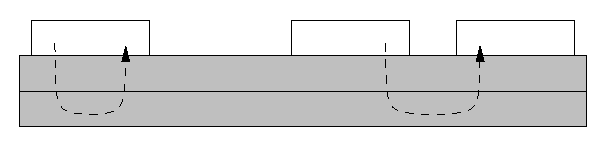
\includegraphics{img/tex/syscall_unx}%
\end{picture}%
\setlength{\unitlength}{4144sp}%
%
\begingroup\makeatletter\ifx\SetFigFont\undefined%
\gdef\SetFigFont#1#2#3#4#5{%
  \reset@font\fontsize{#1}{#2pt}%
  \fontfamily{#3}\fontseries{#4}\fontshape{#5}%
  \selectfont}%
\fi\endgroup%
\begin{picture}(4344,834)(169,-73)
\put(488,584){\makebox(0,0)[lb]{\smash{\SetFigFont{10}{12.0}{\sfdefault}{\mddefault}{\updefault}{\color[rgb]{0,0,0}process}%
}}}
\put(2468,584){\makebox(0,0)[lb]{\smash{\SetFigFont{10}{12.0}{\sfdefault}{\mddefault}{\updefault}{\color[rgb]{0,0,0}process}%
}}}
\put(1576,292){\makebox(0,0)[lb]{\smash{\SetFigFont{10}{12.0}{\sfdefault}{\mddefault}{\updefault}{\color[rgb]{0,0,0}kernel syscall API}%
}}}
\put(2168, 22){\makebox(0,0)[lb]{\smash{\SetFigFont{10}{12.0}{\sfdefault}{\mddefault}{\updefault}{\color[rgb]{0,0,0}kernel}%
}}}
\put(3728,584){\makebox(0,0)[lb]{\smash{\SetFigFont{10}{12.0}{\sfdefault}{\mddefault}{\updefault}{\color[rgb]{0,0,0}process}%
}}}
\end{picture}

\item distributed OS\vspace{1ex}

\begin{picture}(0,0)%
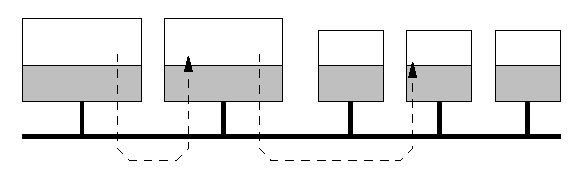
\includegraphics{img/tex/syscall_dist}%
\end{picture}%
\setlength{\unitlength}{4144sp}%
%
\begingroup\makeatletter\ifx\SetFigFont\undefined%
\gdef\SetFigFont#1#2#3#4#5{%
  \reset@font\fontsize{#1}{#2pt}%
  \fontfamily{#3}\fontseries{#4}\fontshape{#5}%
  \selectfont}%
\fi\endgroup%
\begin{picture}(4161,1104)(238,-253)
\put(353,682){\makebox(0,0)[lb]{\smash{\SetFigFont{10}{12.0}{\sfdefault}{\mddefault}{\updefault}{\color[rgb]{0,0,0}u�ivatelsk�}%
}}}
\put(488,547){\makebox(0,0)[lb]{\smash{\SetFigFont{10}{12.0}{\sfdefault}{\mddefault}{\updefault}{\color[rgb]{0,0,0}proces}%
}}}
\put(548,292){\makebox(0,0)[lb]{\smash{\SetFigFont{10}{12.0}{\sfdefault}{\mddefault}{\updefault}{\color[rgb]{0,0,0}j�dro}%
}}}
\put(1568,547){\makebox(0,0)[lb]{\smash{\SetFigFont{10}{12.0}{\sfdefault}{\mddefault}{\updefault}{\color[rgb]{0,0,0}proces}%
}}}
\put(1433,682){\makebox(0,0)[lb]{\smash{\SetFigFont{10}{12.0}{\sfdefault}{\mddefault}{\updefault}{\color[rgb]{0,0,0}u�ivatelsk�}%
}}}
\put(1628,292){\makebox(0,0)[lb]{\smash{\SetFigFont{10}{12.0}{\sfdefault}{\mddefault}{\updefault}{\color[rgb]{0,0,0}j�dro}%
}}}
\put(2596,299){\makebox(0,0)[lb]{\smash{\SetFigFont{10}{12.0}{\sfdefault}{\mddefault}{\updefault}{\color[rgb]{0,0,0}j�dro}%
}}}
\put(2551,569){\makebox(0,0)[lb]{\smash{\SetFigFont{10}{12.0}{\sfdefault}{\mddefault}{\updefault}{\color[rgb]{0,0,0}server}%
}}}
\put(3226,569){\makebox(0,0)[lb]{\smash{\SetFigFont{10}{12.0}{\sfdefault}{\mddefault}{\updefault}{\color[rgb]{0,0,0}server}%
}}}
\put(3271,299){\makebox(0,0)[lb]{\smash{\SetFigFont{10}{12.0}{\sfdefault}{\mddefault}{\updefault}{\color[rgb]{0,0,0}j�dro}%
}}}
\put(3946,299){\makebox(0,0)[lb]{\smash{\SetFigFont{10}{12.0}{\sfdefault}{\mddefault}{\updefault}{\color[rgb]{0,0,0}j�dro}%
}}}
\put(3901,569){\makebox(0,0)[lb]{\smash{\SetFigFont{10}{12.0}{\sfdefault}{\mddefault}{\updefault}{\color[rgb]{0,0,0}server}%
}}}
\end{picture}

\end{itemize}
\end{slide}

\begin{itemize}
\item If a Unix process requires to perform system task, it will pass the
control to the kernel using a system call. The kernel is code shared between
all processes however accessible only to those processes that are running in
kernel mode. The kernel is therefore not a standalone privileged process,
it is still running in the context of a process (one that requested system
service via system call or such that was running when interrupt came).
\item Inter-process communication in UNIX is achieved using system calls,
it is therefore handled by the kernel.
\item There can be system processes called \emph{kernel threads}, that are
running exclusively in kernel mode. The majority of system processes run in user
mode and differ from the rest in that they have elevated privileges.
The process scheduler switches between processes and makes it possible to run
multiple processes simultaneously even on single processor system.
Multi-processor systems enable true parallelism of processes and threads
(it is possible for a thread to migrate between processors based on scheduling).
\item In distributed operating systems the kernel is in the form of microkernel,
i.e. provides only the very basic services like processor programming, memory
allocation and inter-process communication. Upper system services that are part
of kernel in UNIX (e.g. file system access) are implemented as special processes
(servers) running in user mode. The kernel passes the request of user process to
relevant server that can be running on different network node.
\item There are many microkernels today, e.g. Minix (unix-like system) or HURD
that runs above the Mach micro-kernel.
\end{itemize}

%%%%%

\begin{slide}
\sltitle{System calls, functions}
\begin{itemize}
\item In UNIX a distinction is made of \emsl{system calls} and \emsl{library
functions}. This division is maintained in man pages: section \emsl{2} contains
system call man pages and section \emsl{3} library functions.
    \begin{itemize}
    \item library functions are executed in user mode, just like the rest
    of the program's code.
    \item system calls also have the form of a function. However given function
    only processes arguments and passes the control to the kernel using
    synchronous interrupt instruction. Once it returns from the kernel,
    it will adjust the result and returns it to the caller.
    \end{itemize}
\item this distinction is not made in the standard -- from programmer's
perspective it does not \emph{usually} matter if given function is processed
by a library or kernel.
\end{itemize}
\end{slide}

\begin{itemize}
\item The transition from userland to kernel can be costly; if the program
executes lot of syscalls, it can have a negative effect on its performance.
\emsl{Library function can but does not have to perform some system calls,
however it always does some non-trivial work in user mode.}
\item It is possible to perform system call directly in assembler.
\item The kernel API is defined w.r.t. function calls of the standard library,
not w.r.t. interrupt level and data structures used by these functions when
passing control to the kernel. The mechanism of switching between user and
kernel mode can differ not only depending on hardware platform but also between
different versions of the same system on the same hardware.
\end{itemize}

%%%%%

\pdfbookmark[1]{syscall return values semantics}{syscallretvals}

\begin{slide}
\sltitle{System call return values}
\setlength{\baselineskip}{0.8\baselineskip}
\begin{itemize}
\item integer return value (\texttt{int}, \texttt{pid\_t},
\texttt{off\_t}, etc.)
    \begin{itemize}
    \item \texttt{>= 0} \dots{} success
    \item \texttt{== -1} \dots{} failure
    \end{itemize}
\item pointer return value
    \begin{itemize}
    \item \texttt{!= NULL} \dots{} success
    \item \texttt{== NULL} \dots{} failure
    \end{itemize}
\item after failed syscall the error code is stored in global variable
\texttt{extern int \funnm{errno};}
\item successful syscall never changes \texttt{errno} ! It is therefore
necessary to test the return value first and then check \texttt{errno}.
\item error message depending on the \texttt{errno} value can be printed with\\
\texttt{void \funnm{perror}(const char *\emph{s});}
\item textual representation for given value is returned by\\
\texttt{char *\funnm{strerror}(int \emph{errnum});}
\end{itemize}
\end{slide}

%%%%%

\begin{itemize}
\item \label{ERRNO} In Solaris \texttt{errno} is in reality defined in
\texttt{libc} as a dereferenced pointer to integer (specific to userland thread)
and the value is set right after the instruction for system call.
For example on i386 architecture the \texttt{errno} value is stored in the
\texttt{eax} register after the return from the syscall (after the
\texttt{sysenter} instruction is executed). Before the instruction the register
held the system call number. It is therefore the \texttt{libc} library that is
responsible for the program to see the correct \texttt{errno} value.
\item The POSIX thread functions (\texttt{pthread\_*}) do not set
\texttt{errno}, rather they return either zero or error code.
\item For some calls it the \texttt{-1} is semantically valid. To use such
functions, it is necessary to set \texttt{errno~=~0} before the call and check
whether the value changed after the call. E.g. the \texttt{strtol} function
returns 0 on failure, which is valid value even for valid result
(and $-1$ is also valid result value).
\item It is therefore necessary to always read the man page for appropriate
system call or library function.
\item Note that the failure or functions from \texttt{stdio.h} it is necessary
to test using\\
\texttt{int \funnm{ferror}(FILE *\emph{stream})}, because it is not otherwise
possible to distinguish between an error and end of stream. Considering we are
not using these functions in the lecture (except 
\texttt{printf} and \texttt{fprintf} for \texttt{stdout}, resp.
\texttt{stderr}), you should not need it.
\end{itemize}

\begin{slide}
\sltitle{Formatted error messages: \texttt{err(3)}}
\setlength{\baselineskip}{0.8\baselineskip}
\begin{itemize}
\item functions to display a formatted error message and optionally exit
\item instead of \funnm{perror}() and \funnm{exit}(), one function suffices
\item
\texttt{void \funnm{err}(int \emph{status}, const char *\emph{fmt}, ...);}
\begin{itemize}
\item prints a program name, formatted string, and error based on
\texttt{errno}
\item exits the program with \emph{status} return value
\end{itemize}
\item
\texttt{void \funnm{warn}(const char *\emph{fmt}, ...);}
\begin{itemize}
\item same as \funnm{err}() but does not exit
\end{itemize}
\item see the manual page for other functions from the same family
\item originated in 4.4BSD
\end{itemize}
\end{slide}

%%%%%

\begin{itemize}
\label{ERR}
\item The third widely used function is \funnm{errx}() which behaves as
\funnm{err}() but does not use \texttt{errno}.  Similarly, \funnm{warnx}().
\item These functions are very handy especially for smaller programs as they are
easy to work with and save you some lines of code.  More complex
app\-li\-ca\-tions often use their own logging functions.
\item Not part of the UNIX specification but in general you can find them almost
everywhere.
\item Example (and also in \example{err/err.c}):

\begin{verbatim}
#include <errno.h>
#include <err.h>

int
main(void)
{
        errno = 13;
        err(3, "ggr %s", "GRR");
        printf("after err()\n");
        return (0);
}

$ ./a.out 
a.out: ggr GRR: Permission denied
$ echo $?
3
\end{verbatim}

\end{itemize}

\endinput
